\PassOptionsToPackage{hyphens}{url}
\documentclass[11pt,a4paper]{article}
\usepackage[margin=2.2cm]{geometry}
\usepackage{amsmath,amssymb}
\usepackage{graphicx}
\usepackage{booktabs}
\usepackage{tabularx}
\usepackage{float}
\usepackage[font=small,labelfont=bf]{caption}
\usepackage{xcolor}
\usepackage{tikz}
\usetikzlibrary{arrows.meta,calc}
\usepackage{enumitem}
\usepackage[hidelinks]{hyperref}
\setlist{itemsep=2pt,topsep=3pt}
\graphicspath{{figures/}}

\newcommand{\Reng}{R_{\mathrm{eng}}}
\newcommand{\Phit}{P_{\mathrm{hit}}}
\newcommand{\D}{\mathcal{D}}
\newcommand{\obs}[1]{\par\smallskip\noindent\textbf{Observations.} #1\par\smallskip}
\newcommand{\takeaway}[1]{\noindent\textbf{What it shows.} #1\par\medskip}

\title{\textbf{Guardian Point-Defence Fire Control}\\[4pt]
\large Detailed Experimental Report: Predictive Tracking and Turret Control\\ for a Maneuvering Aerial Target (ME 319, Assignment 2)}
\author{[Author Name]\\ Department of Mechanical Engineering, IIT Bombay\\
\small\href{https://github.com/VatshVan/Predictive-Tracking-and-Turret-Control-for-a-Maneuvering-Aerial-Target}{\texttt{github.com/VatshVan/Predictive-Tracking-and-}}\\
\small\href{https://github.com/VatshVan/Predictive-Tracking-and-Turret-Control-for-a-Maneuvering-Aerial-Target}{\texttt{Turret-Control-for-a-Maneuvering-Aerial-Target}}}
\date{November 2026}

\begin{document}
\maketitle

\begin{abstract}
\noindent This report documents every experiment run on the Guardian fire-control design. For each test it records what was done, what was measured, what was observed, and what that means for the design thesis. The thesis has three parts. The prescribed $t_p=0.5$\,s prediction is a lag to be \emph{cancelled}, not a lead. The reference generator returns the predicted reference to the estimated present elevation, with fast, well-damped deviation poles; keeping the full Taylor prediction inside the loop is possible only up to order four and forces slow poles (Section~\ref{sec:research}). And a jerk-state estimator, a plant-inverse feed-forward and a calibrated firing rule then let one frozen design engage any admissible V-44.
Over 1\,000 independent random engagements, the frozen design intercepted every target, bounding its failure probability below 0.38\% (one-sided 97.5\% Wilson). It also intercepted all 1\,000 homotopy-guided adversarial engagements. Of 9\,197 pulses in the main campaign, 99.96\% hit. Interception time follows a slew-limited physical model ($R^2=0.93$). The estimator is statistically consistent ($E[z^2]=1.008$), and the hit probability that drives firing is calibrated. Every design choice is justified by paired, multiplicity-corrected tests, including the ones that went against our expectations.
\end{abstract}

\tableofcontents
\newpage

% ==========================================================================================
\section{Thesis and Hypotheses}
\label{sec:thesis}
The laser is instantaneous, so a hit requires the turret to point at the target's \emph{current} position at the instant of the pulse. The assignment nevertheless prescribes a predicted elevation reference at $t_p=0.5$\,s. Our thesis reconciles the two:

\begin{quote}
\emph{The $t_p$ prediction exists to cancel the lag of the turret loop. A reference generator driven by the predicted reference $A_3(\D)\hat\theta$ can return it exactly to the estimated present elevation, so the turret tracks the target's present elevation. With a jerk-state estimator (matched to the plant's relative degree three), an exact plant-inverse feed-forward and a calibrated hit-probability firing rule, a single frozen design can engage any admissible V-44 trajectory, including through radar loss.}
\end{quote}

\noindent We test six hypotheses that the thesis implies:
\begin{enumerate}[label=\textbf{H\arabic*}]
\item \textbf{Cancellation.} With the prediction-matched reference generator the turret tracks the nowcast. Pointing error is set by the estimator, not by the $t_p$ lead or the loop lag.
\item \textbf{Consistency.} The estimator's covariance is honest, so the hit probability used for firing is calibrated.
\item \textbf{Estimator order.} A jerk-state (order-4) estimator is necessary for maneuver switches and is the robust choice for unseen maneuvers.
\item \textbf{Firing.} The fire-now-or-wait rule wastes almost no pulses and does not delay interception unnecessarily.
\item \textbf{Measurement loss.} Through blackouts up to 0.5\,s the design degrades gracefully, never fires blind late in a loss, and recovers quickly.
\item \textbf{Generalisation.} The frozen design generalises to unseen admissible engagements \emph{and} to the different conventions an unseen evaluation script may use.
\end{enumerate}
Section~\ref{sec:verdict} returns a verdict on each.

% ==========================================================================================
\section{System Under Test}

\begin{figure}[H]
\centering
\resizebox{0.95\textwidth}{!}{%
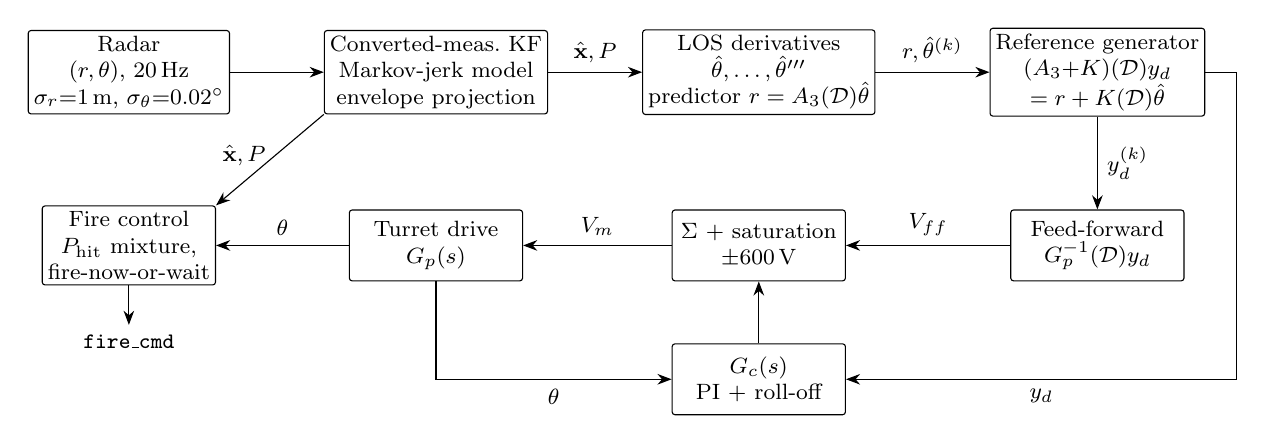
\begin{tikzpicture}[every node/.style={font=\footnotesize},
  blk/.style={draw, rounded corners=1pt, align=center, minimum height=9mm, minimum width=22mm, inner sep=2pt},
  >={Stealth[length=1.8mm]}]
\node[blk] (radar) at (0,0) {Radar\\$(r,\theta)$, 20\,Hz\\$\sigma_r$=1\,m, $\sigma_\theta$=0.02$^\circ$};
\node[blk] (kf) at (3.9,0) {Converted-meas.\ KF\\Markov-jerk model\\envelope projection};
\node[blk] (pred) at (8.0,0) {LOS derivatives\\$\hat\theta,\dots,\hat\theta'''$\\predictor $r=A_3(\D)\hat\theta$};
\node[blk] (ref) at (12.3,0) {Reference generator\\$(A_3{+}K)(\D)y_d$\\$=r+K(\D)\hat\theta$};
\node[blk] (fire) at (0,-2.2) {Fire control\\$\Phit$ mixture,\\fire-now-or-wait};
\node[blk] (plant) at (3.9,-2.2) {Turret drive\\$G_p(s)$};
\node[blk] (sum) at (8.0,-2.2) {$\Sigma$ + saturation\\$\pm600$\,V};
\node[blk] (ff) at (12.3,-2.2) {Feed-forward\\$G_p^{-1}(\D)y_d$};
\node[blk] (gc) at (8.0,-3.9) {$G_c(s)$\\PI + roll-off};
\draw[->] (radar) -- (kf);
\draw[->] (kf) -- node[above]{$\hat{\mathbf x},P$} (pred);
\draw[->] (pred) -- node[above]{$r,\hat\theta^{(k)}$} (ref);
\draw[->] (ref) -- node[right]{$y_d^{(k)}$} (ff);
\draw[->] (ff) -- node[above]{$V_{ff}$} (sum);
\draw[->] (sum) -- node[above]{$V_m$} (plant);
\draw[->] (ref.east) -- ++(0.4,0) |- node[pos=0.75,below]{$y_d$} (gc.east);
\draw[->] (plant.south) |- node[pos=0.75,below]{$\theta$} (gc.west);
\draw[->] (gc) -- (sum);
\draw[->] (kf.south west) -- node[left,pos=0.45]{$\hat{\mathbf x},P$} (fire.north east);
\draw[->] (plant) -- node[above]{$\theta$} (fire);
\draw[->] (fire.south) -- ++(0,-0.5) node[below]{\texttt{fire\_cmd}};
\end{tikzpicture}}
\caption{Architecture of the frozen design. The reference generator contains the predictor polynomial $A_3$, so the $t_p$ lead and the generator lag cancel.}
\label{fig:arch}
\end{figure}

\begin{table}[H]
\centering\small
\caption{Frozen design parameters (identical for every experiment unless a one-factor ablation changes one of them).}
\label{tab:params}
\begin{tabularx}{\textwidth}{@{}lX@{}}
\toprule
Block & Configuration\\
\midrule
Plant & $G_p(s)=1000/[s(320s^2+3350s+1.0015\times10^6)]$; poles $0,\,-5.23\pm55.70j$ (8.90\,Hz, $\zeta=0.094$); supply $\pm600$\,V\\
Estimator & Unbiased converted measurements; per axis $[p,v,a,j]$, jerk Gauss--Markov $\sigma_j=20$\,m/s$^3$, $\tau_j=0.4$\,s; projection $|\mathbf v|\le157.5$, $|\mathbf a|\le23$; $\chi^2$ jump gate 40; class re-identification after loss\\
Predictor & $r=A_3(\D)\hat\theta$, $A_3(s)=1+t_ps+(t_ps)^2/2+(t_ps)^3/6$, $t_p=0.5$\,s\\
Reference generator & $(A_3+K)(\D)y_d=r+K(\D)\hat\theta$, $A_3+K=\tfrac{t_p^3}{6}(s+20)^3$; cascade gains $(p/3,p,3p)$; rate and acceleration limits 0.58\,rad/s, 2.5\,rad/s$^2$\\
Feed-forward & $V_{ff}=0.32\,\dddot y_d+3.35\,\ddot y_d+1001.5\,\dot y_d$\\
Feedback & $G_c(s)=4000(1+1/s)/(0.03s+1)$; conditional-integration anti-windup\\
Fire control & 17 maneuver classes (nominal; $|\mathbf a|=10, 20$\,m/s$^2$ in 8 directions), nominal weight 0.5. Tracking: fire if $\Phit\ge0.99$, or arm at 0.90 and fire at the peak (drop 0.02) or after 0.3\,s. Coasting: fire only while $\Phit\ge0.95$ and falling. Consensus $\ge80\%$ of classes; $\ge8$ radar updates; 1\,s recharge\\
\bottomrule
\end{tabularx}
\end{table}

% ==========================================================================================
\section{Analytical Results}

\subsection{Plant and feedback loop}
\textbf{What we did.} We derived the elevation drive from first principles, computed the open-loop Bode response of $G_cG_p$ (continuous, and with the implemented discrete compensator and a ZOH plant at 100 and 20\,Hz), and simulated the plant's voltage step response and the feedback-only closed loop.

\begin{figure}[H]
\centering
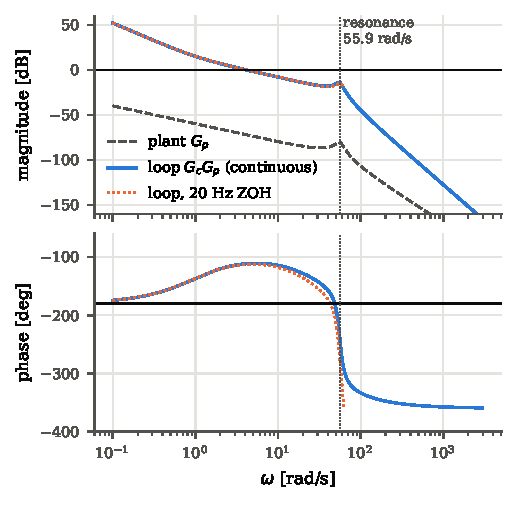
\includegraphics[width=0.48\textwidth]{bode.pdf}
\caption{Bode plot of the plant $G_p$ and the loop $G_cG_p$, continuous and with 20\,Hz ZOH sampling. The dotted line marks the 55.9\,rad/s drive resonance.}
\label{fig:bode}
\end{figure}

\begin{figure}[H]
\centering
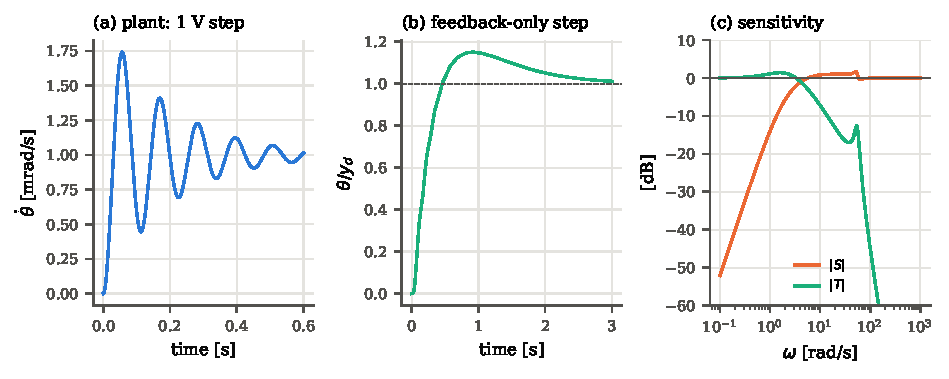
\includegraphics[width=\textwidth]{loop_responses.pdf}
\caption{(a) Turret rate response to a 1\,V step: the 8.9\,Hz electromechanical mode rings with $\zeta=0.094$. (b) Step response of the feedback loop alone (no feed-forward). (c) Sensitivity $|S|$ and complementary sensitivity $|T|$.}
\label{fig:loop}
\end{figure}

\obs{
\begin{itemize}
\item The plant velocity response (Fig.~\ref{fig:loop}a) rings at 8.9\,Hz with very light damping and settles to about 1.0\,mrad/s per volt. Tracking the largest LOS rate in the envelope ($150/800=0.19$\,rad/s) therefore needs about 190\,V, and a $\pm600$\,V supply gives about $3\times$ headroom.
\item The loop crosses over at 4.1\,rad/s with 68.5$^\circ$ phase margin. The resonance peak sits 16.1\,dB below 0\,dB (Fig.~\ref{fig:bode}), so the mode is gain-stabilised without a notch.
\item Sampling barely matters. Margins with the implemented discrete compensator are 68.5$^\circ$/16.1\,dB at 100\,Hz and 67.4$^\circ$/18.6\,dB at 20\,Hz (Table~\ref{tab:margins}).
\item The peak sensitivity is $M_s=1.21$ (1.7\,dB), a very robust loop. The feedback-only step response (Fig.~\ref{fig:loop}b) is well damped, with no visible excitation of the 8.9\,Hz mode.
\end{itemize}}
\takeaway{The feedback loop is deliberately modest and robust. Tracking performance comes from the feed-forward path, not from loop bandwidth (supports H1).}

\begin{table}[H]
\centering\small
\caption{Loop margins of the implemented compensator with ZOH plant.}
\label{tab:margins}
\begin{tabular}{lccc}
\toprule
Sampling & $\omega_c$ [rad/s] & Phase margin [deg] & Gain margin [dB]\\
\midrule
continuous & 4.10 & 68.5 & 16.1\\
1000\,Hz & 4.10 & 68.5 & 16.0\\
100\,Hz & 4.12 & 68.5 & 16.1\\
50\,Hz & 4.14 & 68.4 & 16.3\\
20\,Hz & 4.19 & 67.4 & 18.6\\
\bottomrule
\end{tabular}
\end{table}

\subsection{Prediction-matched reference generator}
\textbf{What we did.} We computed the roots of the Taylor sections $A_n(s)=\sum_{k\le n}(t_ps)^k/k!$ of $e^{st_p}$ for $n=1,\dots,6$. We then compared the transient of the bare prediction-matched lag $1/A_3(s)$ with that of our deviation-feedback design $1/(A_3+K)(s)$.

\begin{figure}[H]
\centering
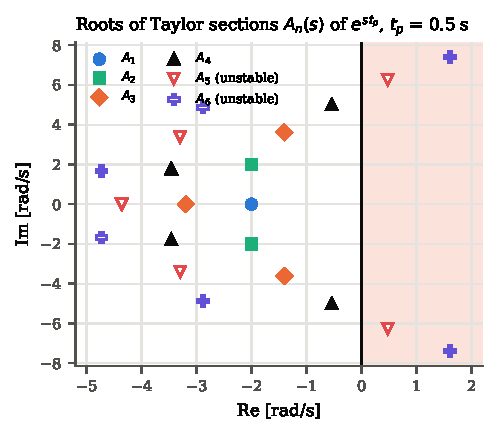
\includegraphics[width=0.47\textwidth]{taylor_roots.pdf}\hfill
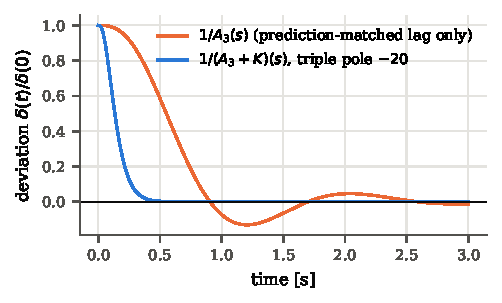
\includegraphics[width=0.5\textwidth]{reference_deviation.pdf}
\caption{Left: roots of the Taylor sections $A_n(s)$. Sections 5 and 6 have right-half-plane roots. Right: decay of a unit deviation $\delta=y_d-\hat\theta$ with the bare prediction-matched lag $1/A_3$ and with the deviation-feedback design (triple pole at $-20$\,rad/s).}
\label{fig:taylor}
\end{figure}

\obs{
\begin{itemize}
\item $A_1$--$A_4$ are Hurwitz; $A_5$ and $A_6$ are not (Fig.~\ref{fig:taylor}, left). The least-damped root has $\zeta=1.00, 0.71, 0.36, 0.11$ for $n=1,\dots,4$.
\item A reference model that exactly cancels a Taylor predictor therefore exists only up to fourth order, and it becomes progressively more oscillatory as the order rises.
\item The bare $1/A_3$ lag decays slowly and overshoots by about 13\% (Fig.~\ref{fig:taylor}, right). In our first prototype, which used it directly, a 0.4\,rad acquisition slew overshot the target by 46\,m and pointing RMS was 5.3\,m.
\item With deviation feedback $K(s)=165.7+24.5s+1.125s^2$, the deviation decays without overshoot in about 0.3\,s, while $y_d\to\hat\theta$ remains exact.
\end{itemize}}
\takeaway{A loop that keeps the full Taylor prediction ($T=1/A_n$) exists only up to order four and is poorly damped. With deviation feedback, $y_d-\hat\theta$ obeys $(\D+20)^3(y_d-\hat\theta)=0$, so the turret still returns to the nowcast, but the Taylor polynomial no longer shapes the loop and the order-4 limit no longer binds. Section~\ref{sec:research} makes this precise and tests the alternatives (supports H1).}

% ==========================================================================================
\section{Experimental Design}

\subsection{Simulation protocol}
The simulator mirrors the evaluation interface. At each controller step $t_k$:
\begin{enumerate}
\item it calls \texttt{target\_motion\_generator}($t_k$);
\item it calls \texttt{turret\_controller}, with the turret state;
\item it judges a pulse on every $0\to1$ edge of \texttt{fire\_cmd} at least 1\,s after the previous pulse: a hit if the target is within 2\,m of the beam ray;
\item it integrates \texttt{turret\_plant} with RK4 at 1\,ms under a zero-order-hold voltage, with mechanical stops at $-10^\circ$ and $+85^\circ$.
\end{enumerate}
Unless stated, the controller runs at 100\,Hz and the turret starts at rest at $0^\circ$.

Metrics:
\begin{itemize}
\item \emph{interception success}: at least one hit;
\item \emph{first-hit time} (the spec's interception time);
\item \emph{pulse hit rate};
\item \emph{pointing RMS}: cross-range $r\sin(\theta-\theta_T)$ over $t\ge2$\,s;
\item \emph{time within $\Reng$};
\item \emph{peak voltage}.
\end{itemize}

\subsection{Standardized and stress scenarios}
\textbf{What we did.} Besides the specification's scenarios A--C, we built six stress scenarios as plausible hidden cases, each targeting one weakness of a predictive fire-control system (Figs.~\ref{fig:scenpaths}--\ref{fig:scenacc}):
\begin{itemize}
\item \textbf{D1} \emph{stealth break}: a $(9,17)$\,m/s$^2$ pull-up that starts \emph{inside} a blackout at 3.0--3.5\,s, the V-44's described tactic.
\item \textbf{D2} \emph{weave}: near-$a_{\max}$ sinusoidal jinking, the worst case for a 0.5\,s predictor.
\item \textbf{D3} \emph{close pass}: the target closes to 853\,m with elevation rising to $83^\circ$, giving peak LOS rate and acceleration near the elevation limit.
\item \textbf{D4} \emph{repeated loss}: scenario B with four blackouts.
\item \textbf{D5} \emph{combined}: weave plus a blackout at short range.
\item \textbf{D6} \emph{jerk test}: $\pm18$\,m/s$^2$ reversals every 1.2\,s with 0.15\,s transitions (450\,m/s$^3$).
\end{itemize}
Every trajectory is generated on a 1\,ms grid and checked against the envelope ($800\le r\le2000$\,m, $|\mathbf v|\le150$\,m/s, $|\mathbf a|\le20$\,m/s$^2$).

\begin{figure}[H]
\centering
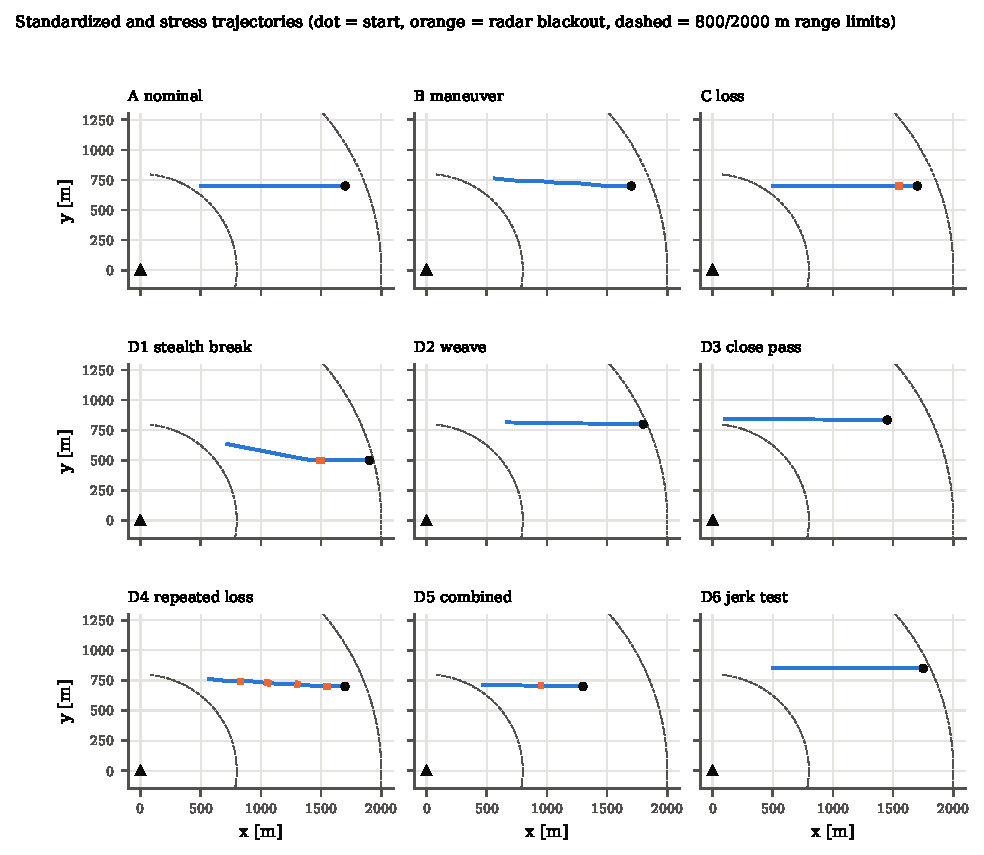
\includegraphics[width=0.92\textwidth]{scenario_paths_grid.pdf}
\caption{Trajectories of the nine scenarios in the elevation plane. Orange segments are radar blackouts.}
\label{fig:scenpaths}
\end{figure}

\begin{figure}[H]
\centering
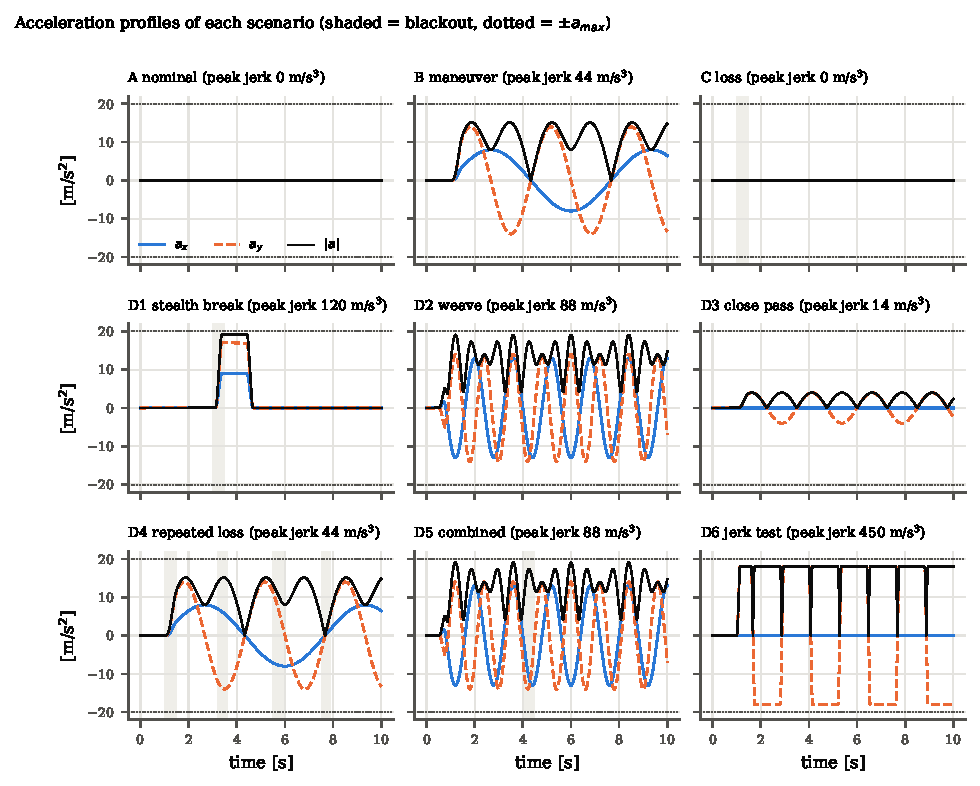
\includegraphics[width=0.92\textwidth]{scenario_accel_grid.pdf}
\caption{Acceleration profiles and peak jerk of each scenario. Shading marks blackouts.}
\label{fig:scenacc}
\end{figure}

\subsection{Monte Carlo engagements}
\textbf{What we did.} Each seed draws one random admissible engagement:
\begin{itemize}
\item initial range $U(1500,2000)$\,m, elevation $U(8^\circ,55^\circ)$, speed $U(70,150)$\,m/s, and an inbound heading within $\pm40^\circ$;
\item maneuver onset at $U(0.5,3)$\,s, then per axis a sum of three sinusoids (frequency $U(0.1,1)$\,Hz, random phase and amplitude), plus with probability 0.5 a smooth ``break'' pulse;
\item the whole profile scaled to a peak of $U(0.4,1)\times0.97\,a_{\max}$;
\item one blackout with onset $U(1,8.5)$\,s and duration $U(0.1,0.5)$\,s, and with probability 0.3 a second one.
\end{itemize}
Inadmissible draws are rejected. Radar noise uses an independent stream per seed.

\begin{figure}[H]
\centering
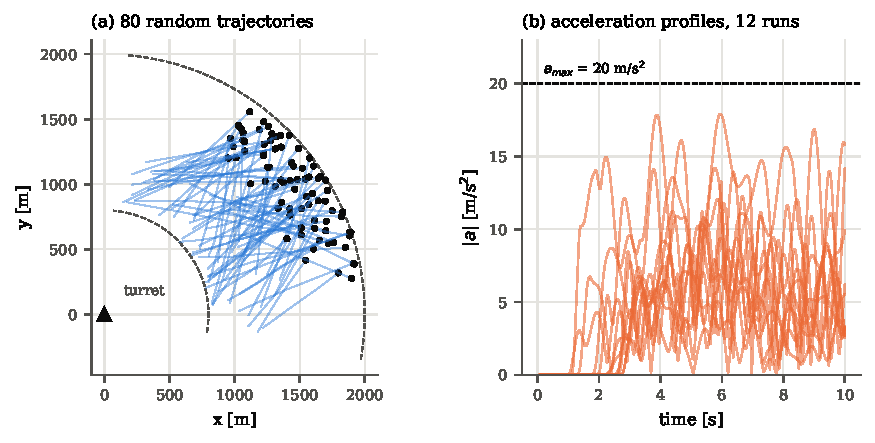
\includegraphics[width=0.92\textwidth]{mc_paths.pdf}
\caption{(a) Eighty sampled Monte Carlo trajectories. (b) Acceleration magnitude of twelve runs.}
\label{fig:mcpaths}
\end{figure}

\begin{figure}[H]
\centering
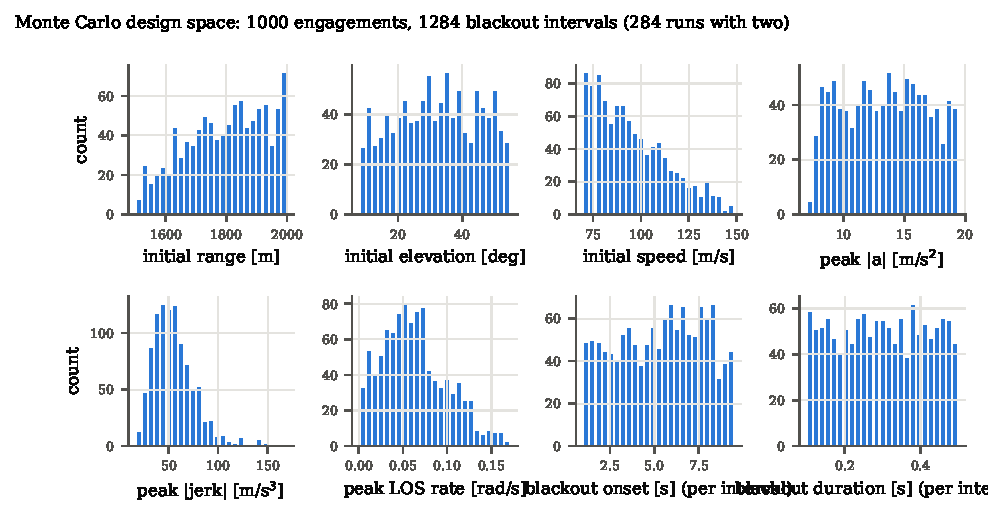
\includegraphics[width=0.95\textwidth]{mc_features.pdf}
\caption{Realised design space over the 1\,000 baseline engagements.}
\label{fig:mcfeat}
\end{figure}

\obs{
\begin{itemize}
\item The 1\,000 engagements span initial ranges of 1500--2000\,m, elevations of 8--55$^\circ$, speeds of 70--150\,m/s, peak acceleration of 7.0--19.4\,m/s$^2$, peak jerk of 17--169\,m/s$^3$ and peak LOS rate up to 0.171\,rad/s.
\item There are 1\,284 blackout intervals (716 runs with one, 284 with two), with onsets spread over 1--9.5\,s and durations over 0.1--0.5\,s (Fig.~\ref{fig:mcfeat}).
\item The generator's jerk tops out near 170\,m/s$^3$, well below D6's 450\,m/s$^3$. This is why the stress noise ensembles (Section~\ref{sec:stress}) are needed alongside the Monte Carlo.
\end{itemize}}

\subsection{Statistical methodology}
\begin{itemize}
\item \emph{Proportions} (interception, pulse hits): Wilson score 95\% intervals. Pulse hit rates also get a cluster bootstrap over engagements (10\,000 resamples), because pulses within one engagement are correlated.
\item \emph{Continuous metrics}: percentile bootstrap 95\% intervals.
\item \emph{Design comparisons}: \textbf{paired} on identical seeds (same trajectory, blackouts and noise), using
  \begin{itemize}
  \item Wilcoxon signed-rank tests (Pratt zero handling) for first-hit time and pointing RMS;
  \item a sign-flip permutation test (20\,000 permutations) for per-run missed pulses;
  \item an exact McNemar test for interception;
  \item Holm--Bonferroni correction within each metric family.
  \end{itemize}
\item \emph{Estimator consistency}: the normalised error $z=e/\hat\sigma$ is compared with $\mathcal N(0,1)$.
\item \emph{Firing calibration}: a reliability diagram and Brier score for $\Phit$.
\item All random draws use fixed seeds.
\end{itemize}

% ==========================================================================================
\section{Results I: Individual Scenarios}
\textbf{What we did.} We ran each scenario once at 1\,kHz with the frozen design. Each figure shows four panels:
\begin{enumerate}
\item true, estimated and $t_p$-predicted elevation and the turret angle;
\item cross-range pointing error, with the $\pm2$\,m band and each pulse marked;
\item motor voltage;
\item the predicted hit probability $\Phit$.
\end{enumerate}

\begin{table}[H]
\centering\small
\caption{Scenario results (single realisation, 1\,kHz controller).}
\label{tab:scen}
\begin{tabular}{llcccc}
\toprule
ID & Description & First hit [s] & Pulses hit & Pointing RMS [m] & Time in $\Reng$\\
\midrule
A & nominal & 1.00 & 9/9 & 0.32 & 100\%\\
B & maneuvering & 1.00 & 9/9 & 0.53 & 100\%\\
C & radar loss 1.0--1.5\,s & 0.98 & 10/10 & 0.41 & 100\%\\
D1 & stealth break & 0.71 & 10/10 & 0.40 & 100\%\\
D2 & weave & 1.02 & 9/9 & 0.99 & 96.3\%\\
D3 & close pass to $83^\circ$ & 1.27 & 9/9 & 0.32 & 100\%\\
D4 & four blackouts & 0.97 & 9/9 & 0.59 & 100\%\\
D5 & weave + blackout & 1.16 & 9/9 & 0.69 & 100\%\\
D6 & jerk test & 1.10 & 8/9 & 0.78 & 98.1\%\\
\bottomrule
\end{tabular}
\end{table}

\begin{figure}[H]
\centering
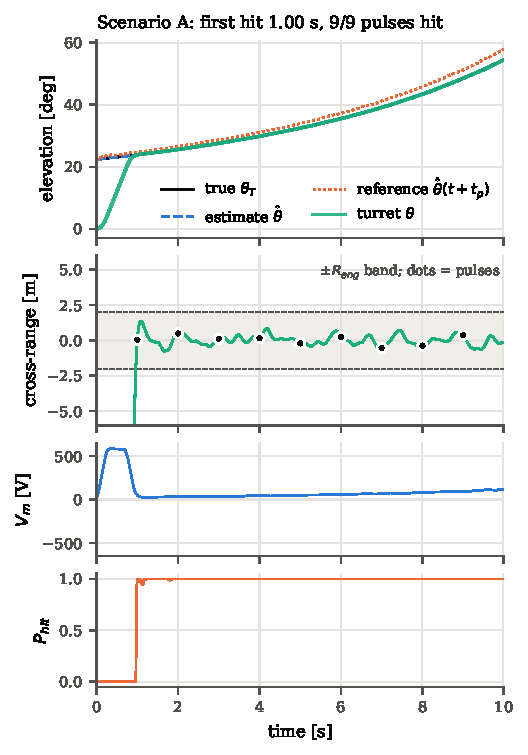
\includegraphics[width=0.48\textwidth]{scenario_A.pdf}\hfill
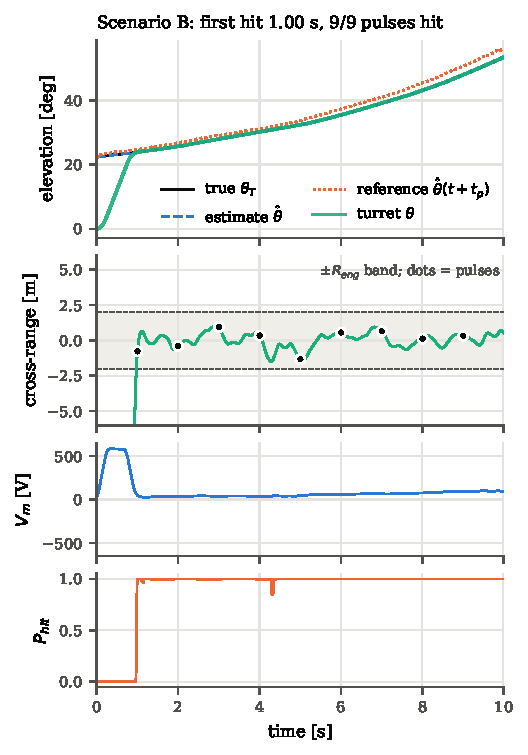
\includegraphics[width=0.48\textwidth]{scenario_B.pdf}
\caption{Scenario A (left) and Scenario B (right).}
\label{fig:AB}
\end{figure}

\obs{
\begin{itemize}
\item \textbf{Acquisition (A, B).} The turret starts at $0^\circ$ with the target at $22^\circ$. The drive saturates at about 583\,V for about 0.7\,s while the reference generator's rate limit (0.58\,rad/s) governs the slew. It then settles onto the target without overshoot and fires the first pulse at 1.00\,s.
\item \textbf{The $t_p$ lead.} The orange predicted reference runs visibly \emph{ahead} of the true elevation by about $t_p$ throughout, while the turret (green) sits on the true elevation. This is the cancellation of H1 made visible.
\item \textbf{A, steady state.} Pointing error stays within $\pm0.8$\,m. Voltage rises slowly from about 30 to 110\,V as the closing target's LOS rate grows. Every pulse lands within 0.6\,m of the centre.
\item \textbf{B, maneuvering.} The sinusoidal maneuver causes excursions up to 1.5\,m, and $\Phit$ dips to 0.85 at 4.3\,s, coinciding with an acceleration reversal. No pulse is fired during the dip. All 9 pulses hit.
\end{itemize}}

\begin{figure}[H]
\centering
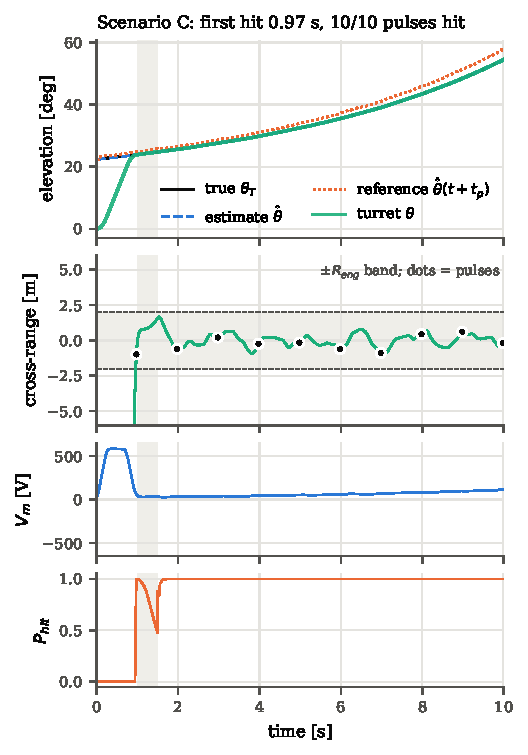
\includegraphics[width=0.48\textwidth]{scenario_C.pdf}\hfill
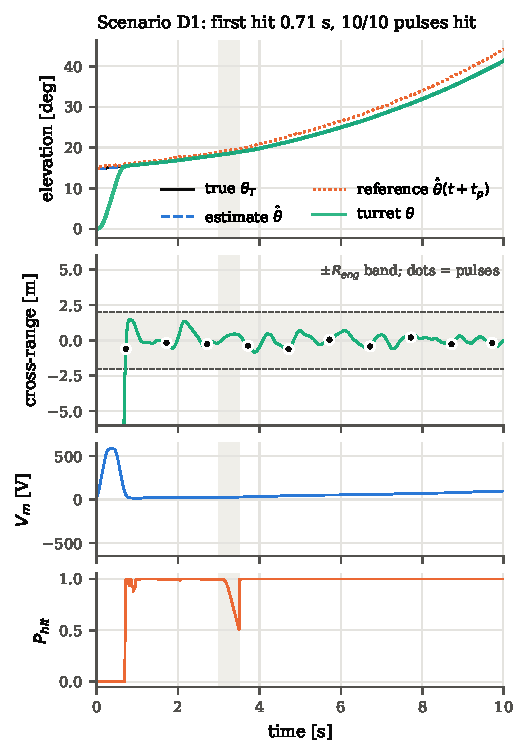
\includegraphics[width=0.48\textwidth]{scenario_D1.pdf}
\caption{Scenario C (left) and stress scenario D1, stealth break (right). Shading marks the blackout.}
\label{fig:CD1}
\end{figure}

\obs{
\begin{itemize}
\item \textbf{C.} The blackout starts at 1.0\,s, just as the turret finishes acquisition. The first pulse fires at 0.98\,s, \emph{before} the loss. During the loss $\Phit$ decays smoothly to about 0.35, reflecting the coasting covariance, and the firing rule holds fire. Pointing error briefly reaches 2.6\,m at 1.5\,s, because the track was only 1\,s old when coasting began. After recovery the error returns inside 1\,m within about 0.4\,s, and every later pulse hits.
\item \textbf{D1.} The target pulls up at about 19\,m/s$^2$ \emph{while unobserved}. The coasted estimate keeps the actual pointing error within about $\pm0.5$\,m because the maneuver ramps in over 0.3\,s, yet $\Phit$ honestly falls to about 0.5 by the end of the loss. Fire was held: the pulse cadence (2.72\,s, then 3.72\,s) skips the blackout. All 10 pulses hit. The first hit comes at 0.71\,s because the initial slew is only $15^\circ$.
\end{itemize}}

\begin{figure}[H]
\centering
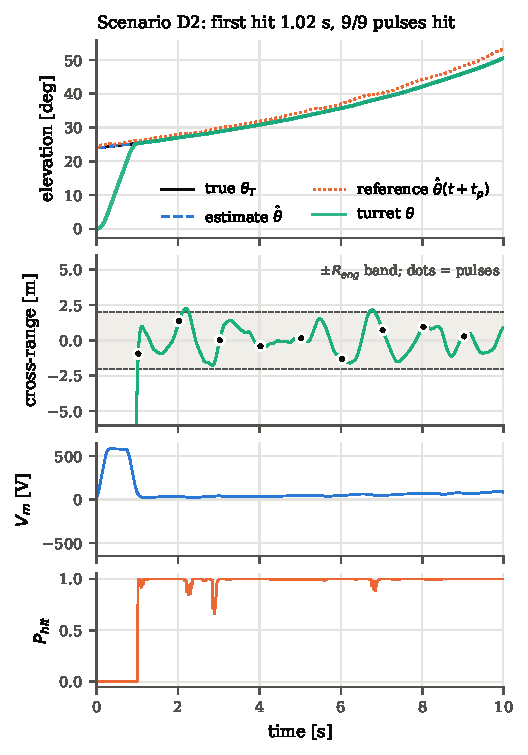
\includegraphics[width=0.48\textwidth]{scenario_D2.pdf}\hfill
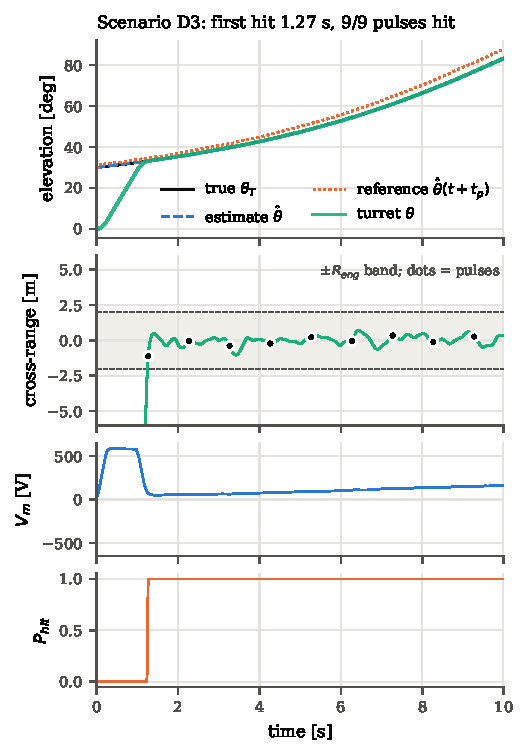
\includegraphics[width=0.48\textwidth]{scenario_D3.pdf}
\caption{Stress scenarios D2, weave (left) and D3, close pass (right).}
\label{fig:D2D3}
\end{figure}

\obs{
\begin{itemize}
\item \textbf{D2.} This is the hardest pointing case. The near-$a_{\max}$ weave drives the error to $\pm2.2$\,m \emph{between} pulses, at about 2.2, 2.7 and 6.8\,s, where $\Phit$ drops to 0.67--0.85. The fire-now-or-wait rule never fires at those moments: every pulse lands within 1.4\,m. This is the clearest demonstration of the firing logic (H4).
\item \textbf{D3.} The elevation climbs to $83^\circ$ and the LOS rate peaks near the end, so the voltage rises to about 160\,V. This is the highest steady demand of any scenario, still far below the 600\,V limit. Tracking is the tightest of all (about $\pm0.6$\,m), and $\Phit$ stays near 1.
\end{itemize}}

\begin{figure}[H]
\centering
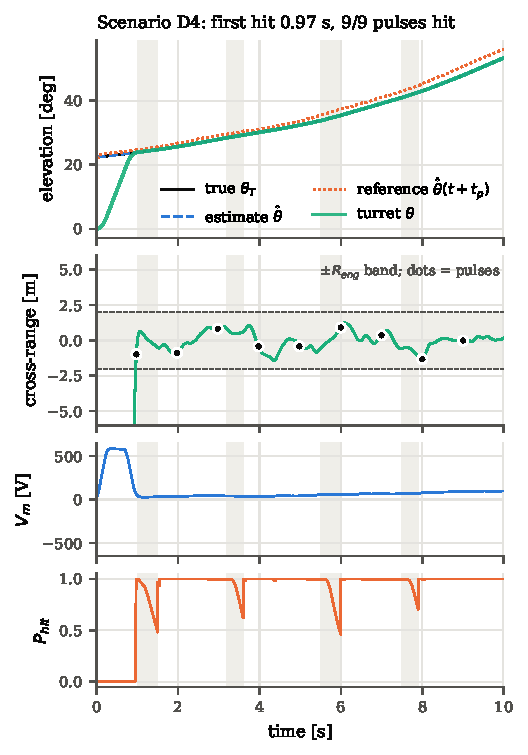
\includegraphics[width=0.48\textwidth]{scenario_D4.pdf}\hfill
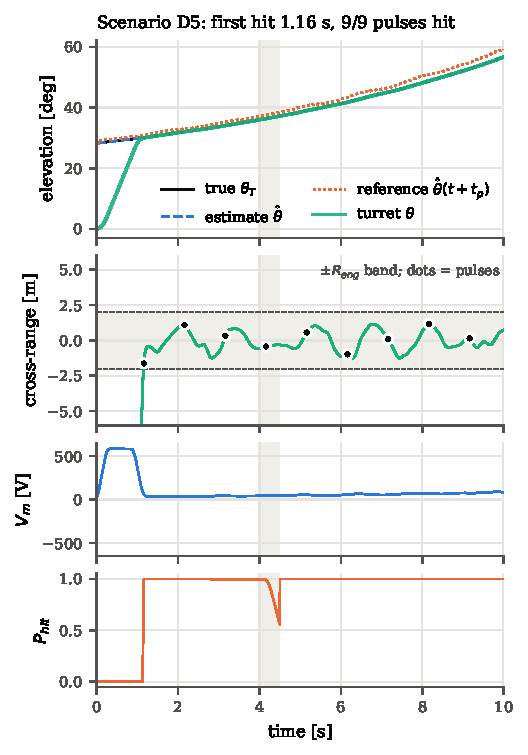
\includegraphics[width=0.48\textwidth]{scenario_D5.pdf}
\caption{Stress scenarios D4, four blackouts (left) and D5, weave plus blackout (right).}
\label{fig:D4D5}
\end{figure}

\obs{
\begin{itemize}
\item \textbf{D4.} Each of the four blackouts produces the same signature: $\Phit$ decays to 0.47--0.70, fire is held, and $\Phit$ snaps back to about 1 at the first returning measurement. Pointing error stays within $\pm1.4$\,m throughout, and all 9 pulses hit.
\item \textbf{D5.} A pulse fires at about 4.15\,s, \emph{inside} the blackout. The rule allowed it because $\Phit$ was still above 0.95 early in the loss, and it hit at 0.4\,m. This is the ``fire just after the loss starts'' behaviour working as intended (H5).
\end{itemize}}

\begin{figure}[H]
\centering
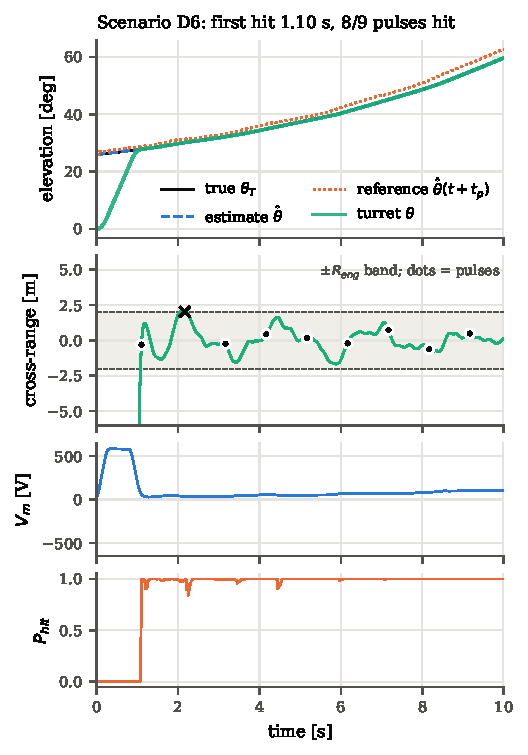
\includegraphics[width=0.48\textwidth]{scenario_D6.pdf}
\caption{Stress scenario D6, jerk test.}
\label{fig:D6}
\end{figure}

\obs{
\begin{itemize}
\item D6 reverses $\pm18$\,m/s$^2$ every 1.2\,s. The order-4 estimator follows each reversal, holding 98.1\% of the time within $\Reng$.
\item In this one realisation, the second pulse, at 2.1\,s just after the first reversal, was fired at $\Phit=0.9901$ and missed by 2\,cm: the estimate error ($+0.93$\,m, about $2.4\sigma$) and the turret lag ($+1.09$\,m) added up in the same direction.
\item Across 50 independent noise realisations of D6 (Section~\ref{sec:stress}), the final design missed \emph{none} of its D6 pulses. This miss is a single unlucky draw, not a systematic weakness.
\end{itemize}}

% ==========================================================================================
\section{Results II: Monte Carlo Campaign (1\,000 engagements)}

\subsection{Interception and engagement accuracy}
\begin{table}[H]
\centering\small
\caption{Final design over 1\,000 random admissible engagements (100\,Hz).}
\label{tab:mc}
\begin{tabular}{lll}
\toprule
Metric & Value & 95\% interval\\
\midrule
Interceptions & 1000/1000 & [99.62\%, 100\%]; failure $<0.38\%$\\
Pulse hit rate & 99.96\% (4 misses / 9\,197) & [99.91, 99.99]\% (cluster bootstrap)\\
First-hit time, mean & 1.214\,s & [1.190, 1.239]\,s\\
First-hit time, p95 / max & 1.83\,s / 2.14\,s & \\
Pointing RMS, median / p95 & 0.559\,m / 0.828\,m & \\
Time within $\Reng$ & 99.40\% & \\
Peak voltage & 589\,V & limit 600\,V\\
\bottomrule
\end{tabular}
\end{table}

\begin{figure}[H]
\centering
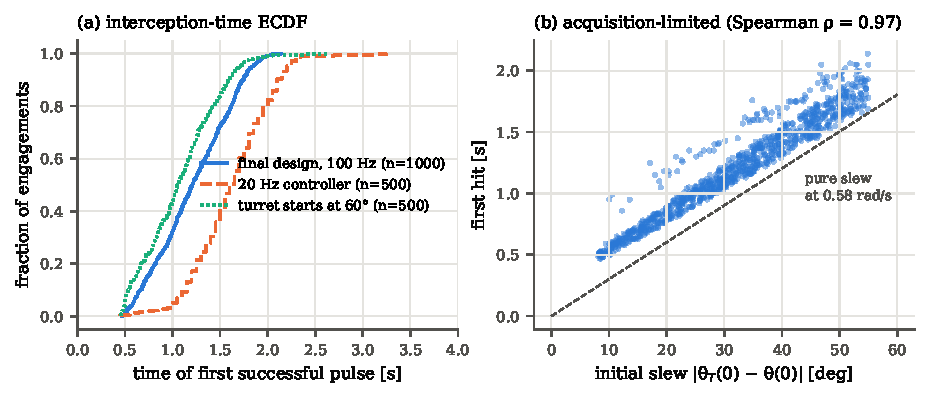
\includegraphics[width=\textwidth]{mc_first_hit.pdf}
\caption{(a) Interception-time ECDFs for the final design (100\,Hz), a 20\,Hz controller and a turret starting at $60^\circ$. (b) First-hit time against the initial slew angle; the dashed line is a pure slew at the 0.58\,rad/s limit.}
\label{fig:fh}
\end{figure}

\obs{
\begin{itemize}
\item Every engagement was intercepted. 50\% are intercepted by about 1.2\,s and all by 2.14\,s (Fig.~\ref{fig:fh}a).
\item Interception time is almost entirely explained by the initial slew angle (Fig.~\ref{fig:fh}b, Spearman $\rho=0.97$). A least-squares fit gives
\[ t_{\mathrm{hit}} \approx 0.263\,\mathrm{s} + 0.0296\,\tfrac{\mathrm s}{\mathrm{deg}}\times\text{slew}, \qquad R^2=0.93,\ \text{residual s.d. } 0.10\,\mathrm s. \]
The slope corresponds to a 0.589\,rad/s slew, matching the 0.58\,rad/s reference-generator limit.
\item The intercept (about 0.26\,s) is settling plus the 8-update firing gate. Targets needing under $10^\circ$ of slew are intercepted at 0.51\,s on average.
\item First-hit time is \emph{not} significantly correlated with maneuver intensity (RMS acceleration $\rho=0.05$, $p=0.15$), peak jerk ($\rho=0.03$) or blackout time ($\rho=0.05$, $p=0.09$).
\item Starting the turret at $60^\circ$ shortens interception (mean 1.07\,s), because most targets sit between $8^\circ$ and $55^\circ$. A 20\,Hz controller lengthens it (mean 1.62\,s).
\end{itemize}}
\takeaway{Interception time is set by turret kinematics, not by estimation or by the target. It can be \emph{predicted} for an unseen case from its geometry (used in Section~\ref{sec:final}).}

\begin{figure}[H]
\centering
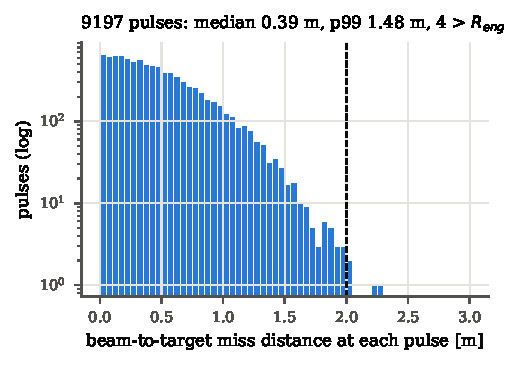
\includegraphics[width=0.55\textwidth]{mc_miss_hist.pdf}
\caption{Beam-to-target miss distance at all 9\,197 pulses (log scale).}
\label{fig:miss}
\end{figure}

\begin{figure}[H]
\centering
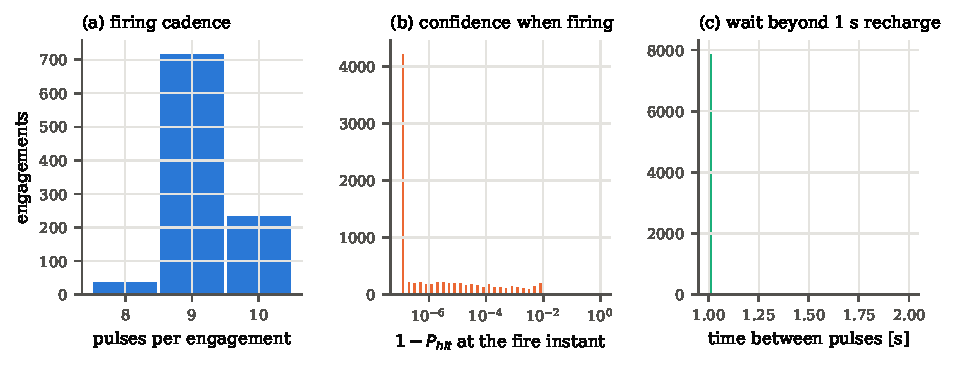
\includegraphics[width=\textwidth]{mc_pulses.pdf}
\caption{(a) Pulses per engagement. (b) $1-\Phit$ at the fire instant. (c) Time between consecutive pulses.}
\label{fig:pulses}
\end{figure}

\obs{
\begin{itemize}
\item \textbf{Miss distances} decay roughly exponentially (Fig.~\ref{fig:miss}): median 0.39\,m, 90th percentile 0.95\,m, 99th percentile 1.48\,m. Only 4 of 9\,197 pulses exceed 2\,m, all by 1--26\,cm, and all are tracking shots.
\item \textbf{Cadence.} Engagements fire 8--10 pulses (mean 9.2; Fig.~\ref{fig:pulses}a), close to the maximum allowed by the 1\,s recharge after acquisition. 65\% of follow-up pulses fire within 10\,ms of the recharge completing, and 95\% within 10\,ms (Fig.~\ref{fig:pulses}c), so the wait-for-a-better-shot option is used sparingly.
\item \textbf{Confidence.} 89.7\% of pulses were fired at $\Phit\ge0.999$ (Fig.~\ref{fig:pulses}b). 211 of 9\,197 pulses were coasting shots (early in a blackout), and none of them missed.
\end{itemize}}
\takeaway{The firing rule converts tracking accuracy into hits with almost no waste, and it does so without slowing the cadence (supports H4).}

\subsection{Pointing accuracy over time}
\begin{figure}[H]
\centering
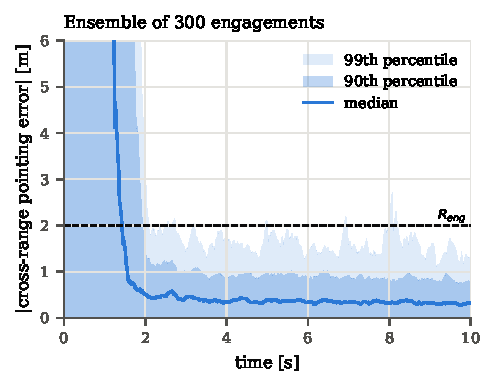
\includegraphics[width=0.52\textwidth]{mc_error_bands.pdf}
\caption{Cross-range pointing error over 300 logged engagements: median, 90th and 99th percentiles.}
\label{fig:bands}
\end{figure}

\begin{figure}[H]
\centering
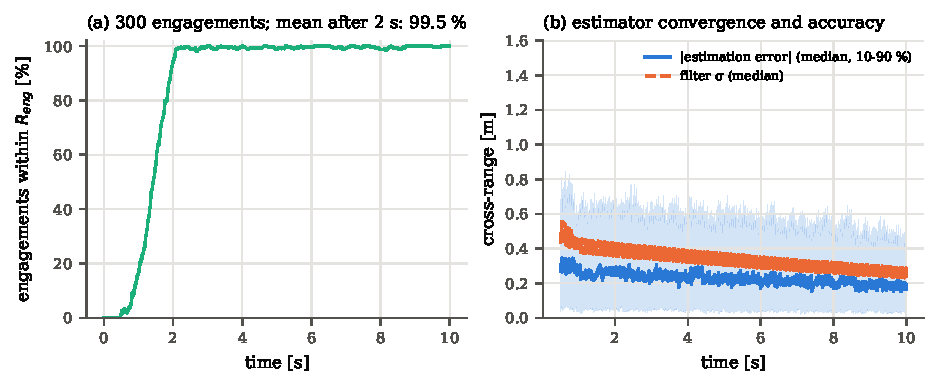
\includegraphics[width=\textwidth]{mc_ensemble_extras.pdf}
\caption{(a) Fraction of engagements pointing within $\Reng$ over time. (b) Estimation error and filter $\sigma$ over time (medians, 10--90\% band).}
\label{fig:ensx}
\end{figure}

\obs{
\begin{itemize}
\item The median pointing error drops below 2\,m at 1.43\,s, and the 90th percentile at 1.93\,s (Fig.~\ref{fig:bands}). After 2\,s the median settles near 0.35\,m and the 90th percentile below 1\,m.
\item The 99th percentile exceeds 2\,m only in brief spikes, which correspond to blackout recoveries.
\item After 2\,s, 99.5\% of engagement-time is within $\Reng$ (Fig.~\ref{fig:ensx}a).
\item The estimator converges within about 1\,s. Afterwards the median cross-range estimation error is 0.22\,m against a median filter $\sigma$ of 0.32\,m (Fig.~\ref{fig:ensx}b), far below the 0.7\,m cross-range noise of a single radar sample at 2\,km.
\end{itemize}}
\takeaway{Pointing error is set by the estimator, about 0.2--0.4\,m, as H1 predicts: the $t_p$ lead and the loop lag add essentially nothing in steady tracking.}

\begin{figure}[H]
\centering
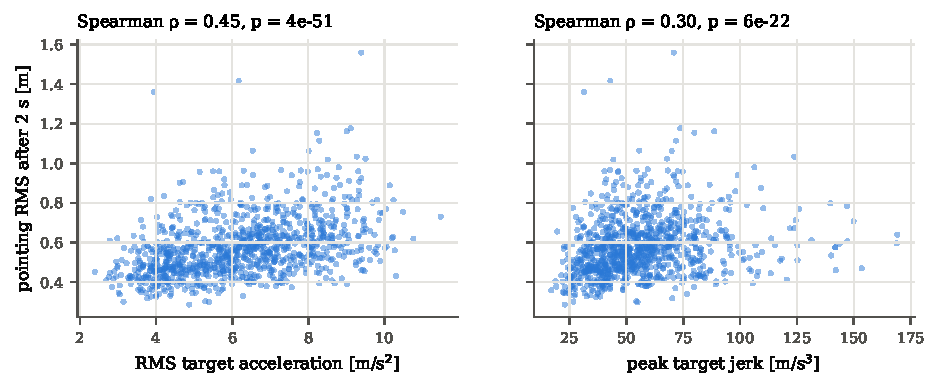
\includegraphics[width=\textwidth]{mc_difficulty.pdf}
\caption{Pointing RMS against RMS target acceleration and peak target jerk.}
\label{fig:diff}
\end{figure}

\obs{
\begin{itemize}
\item Pointing accuracy degrades gracefully and monotonically with maneuver intensity: Spearman $\rho=0.45$ with RMS acceleration and $\rho=0.30$ with peak jerk, both highly significant (Fig.~\ref{fig:diff}).
\item Even the hardest engagements stay below 1.6\,m RMS. The few outliers at low acceleration are engagements with long or double blackouts early in the track.
\end{itemize}}

\subsection{Behaviour across radar loss}
\begin{figure}[H]
\centering
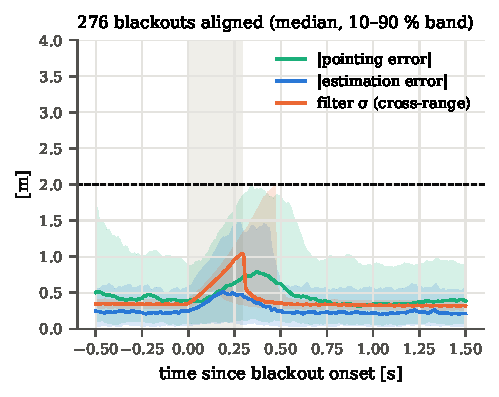
\includegraphics[width=0.6\textwidth]{mc_blackout_aligned.pdf}
\caption{Errors and filter $\sigma$ for 276 blackouts aligned at onset (median, 10--90\% band; median blackout duration shaded).}
\label{fig:bo}
\end{figure}

\obs{
\begin{itemize}
\item \textbf{Before the loss}, the median pointing error is about 0.4\,m and the median $\sigma$ about 0.35\,m.
\item \textbf{During the loss}, the filter's $\sigma$ grows fastest, to about 1.0\,m at 0.3\,s, because it allows for every admissible maneuver. The actual estimation error grows more slowly (median about 0.5\,m), and pointing error lags it (median peak about 0.8\,m at about 0.35\,s).
\item The 90th-percentile band reaches about 2\,m only at the end of the longest losses. This is consistent with the $\tfrac12a_{\max}t^2=2.5$\,m worst-case drift in 0.5\,s.
\item \textbf{On recovery}, the first measurement collapses $\sigma$ immediately, and pointing returns to its pre-loss level within about 0.4\,s, set by the reference generator's triple pole at $-20$\,rad/s.
\end{itemize}}
\takeaway{The system degrades gracefully, its uncertainty grows honestly (and conservatively), and it recovers fast (supports H5).}

\subsection{Estimator consistency and firing calibration}
\begin{figure}[H]
\centering
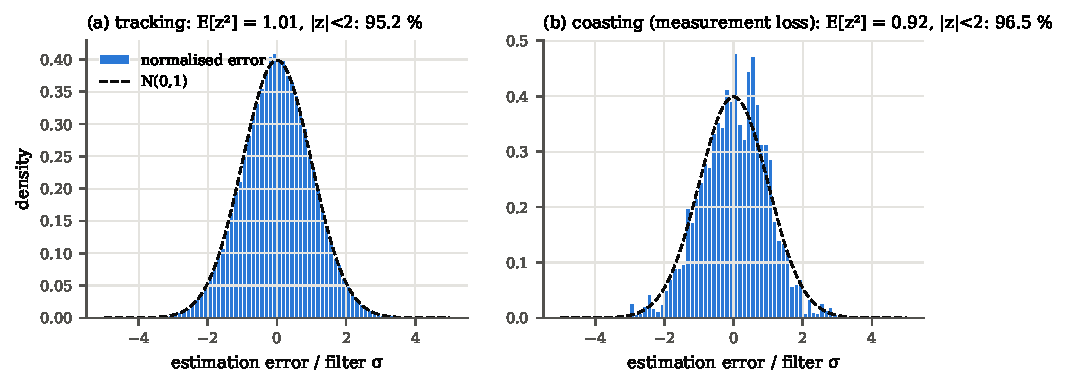
\includegraphics[width=\textwidth]{mc_consistency.pdf}
\caption{Normalised estimation error $z=e/\hat\sigma$ against $\mathcal N(0,1)$: (a) tracking, (b) coasting.}
\label{fig:cons}
\end{figure}

\begin{figure}[H]
\centering
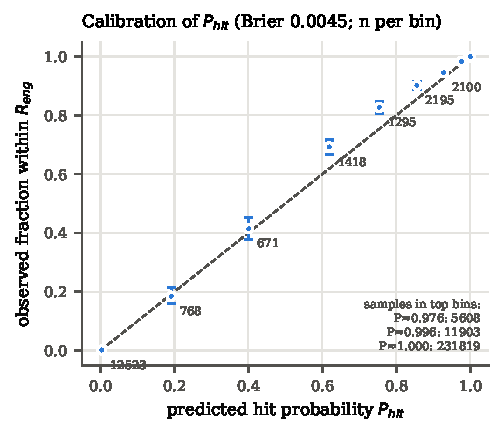
\includegraphics[width=0.5\textwidth]{mc_calibration.pdf}
\caption{Reliability diagram of the predicted hit probability (about 270\,000 controller samples; Wilson 95\% intervals).}
\label{fig:cal}
\end{figure}

\obs{
\begin{itemize}
\item \textbf{Tracking.} The normalised error is almost exactly standard normal: $E[z^2]=1.008$ (ideal 1), with 95.2\% of samples within $|z|<2$ (ideal 95.4\%).
\item \textbf{Coasting.} The distribution is narrower: $E[z^2]=0.92$, 96.5\% within $|z|<2$. During losses the filter is slightly conservative, which is the safe direction.
\item \textbf{Calibration.} Observed hit frequency follows the predicted $\Phit$ in every bin, with a Brier score of 0.0045 (Fig.~\ref{fig:cal}). In the mid-range bins the observed frequency is \emph{higher} than predicted (0.62$\to$0.69, 0.75$\to$0.83).
\item At the 9\,197 fire instants, the mean predicted $\Phit$ implied 8.6 expected misses; 4 occurred.
\end{itemize}}
\takeaway{The probabilities driving the firing decision are honest and slightly conservative (supports H2).}

% ==========================================================================================
\section{Results III: Design Decisions under Paired Statistics}

\subsection{One-factor ablations (500 paired seeds)}
\textbf{What we did.} Each design choice was reverted or perturbed one at a time and run on the same 500 seeds as the final design.

\begin{figure}[H]
\centering
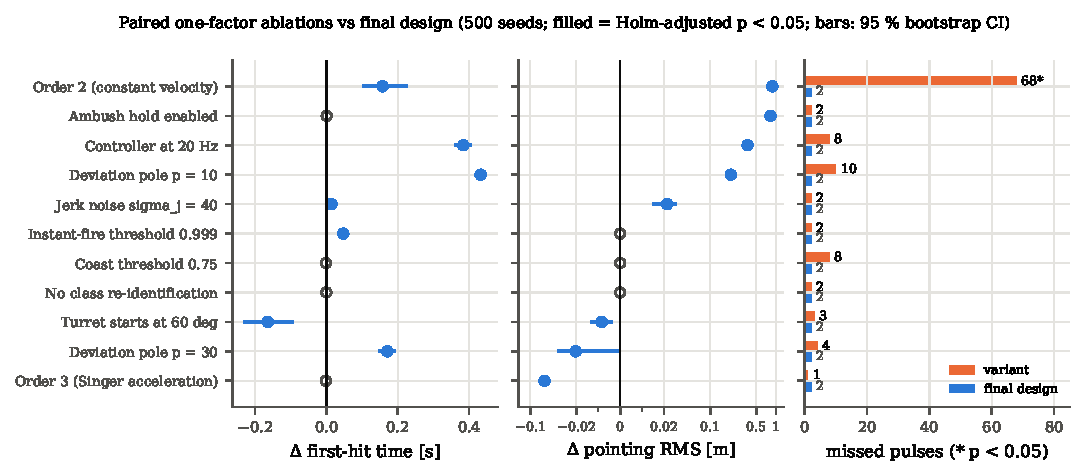
\includegraphics[width=\textwidth]{mc_ablation_forest.pdf}
\caption{Paired ablations: mean paired difference (variant minus final) with 95\% bootstrap CI; filled markers have Holm-adjusted $p<0.05$. Right: missed pulses.}
\label{fig:forest}
\end{figure}

\begin{table}[H]
\centering\footnotesize
\caption{Paired ablations (variant minus final; Holm-adjusted $p$).}
\label{tab:abl}
\begin{tabularx}{\textwidth}{@{}Xllll@{}}
\toprule
Variant & $\Delta$ first hit [s], $p$ & $\Delta$ pointing RMS [m], $p$ & Misses final$\to$var. & Verdict\\
\midrule
Order 2 (constant velocity) & $+0.157$, $5\times10^{-43}$ & $+0.878$, $10^{-74}$ & 2$\to$68; 3 int.\ lost & strongly worse\\
Deviation pole $p=10$ & $+0.433$, $2\times10^{-82}$ & $+0.206$, $10^{-82}$ & 2$\to$10 & strongly worse\\
Ambush hold on & $+0.001$, 1 & $+0.822$, $6\times10^{-51}$ & 2$\to$2 & rejected\\
Controller at 20\,Hz & $+0.384$, $6\times10^{-78}$ & $+0.369$, $10^{-82}$ & 2$\to$8 & slower, still 500/500\\
Deviation pole $p=30$ & $+0.171$, $10^{-31}$ & $-0.021$, $3\times10^{-49}$ & 2$\to$4 & slower for a marginal gain\\
Instant-fire 0.999 & $+0.047$, $2\times10^{-36}$ & 0 & 2$\to$2 & slower, no gain: rejected\\
Jerk noise $\sigma_j=40$ & $+0.014$, 0.0013 & $+0.022$, $3\times10^{-10}$ & 2$\to$2 & slightly worse\\
Coast threshold 0.75 & $-0.002$, 0.63 & 0 & 2$\to$8 ($p=0.65$) & more misses (n.s.)\\
No class re-identification & 0, 1 & 0, 0.77 & 2$\to$2 & no measurable effect\\
Order 3 (Singer) & $-0.002$, 1 & $-0.061$, $5\times10^{-70}$ & 2$\to$1 & better on smooth MC\\
Turret starts at $60^\circ$ & $-0.165$, $2\times10^{-5}$ & $-0.008$, 0.0024 & 2$\to$3 & shorter slew\\
\bottomrule
\end{tabularx}
\end{table}

\obs{
\begin{itemize}
\item \textbf{Estimator order matters most.} A constant-velocity filter (order 2) more than doubles pointing RMS, multiplies misses by 34 and loses 3 interceptions.
\item \textbf{The deviation pole is a genuine trade-off.} At $p=10$, corrections are absorbed slowly, so interception is 0.43\,s later and pointing 0.21\,m worse. At $p=30$, acquisition is 0.17\,s slower, because the cascade saturates longer, for only 0.02\,m better pointing. $p=20$ sits at the knee.
\item \textbf{Two of our own ideas did not survive.} The ambush hold (park the beam where every maneuver class must cross) worsened pointing by 0.82\,m with no extra hits. Class re-identification at recovery had no measurable effect, because the Kalman update with the coasted covariance already performs that correction. We report both rather than claim them.
\item \textbf{Firing thresholds.} 0.999 instead of 0.99 delays interception with identical misses. A coast threshold of 0.75 instead of 0.95 quadruples misses on these seeds, though not significantly at this sample size.
\end{itemize}}

\subsection{Stress-scenario noise ensembles}
\label{sec:stress}
\textbf{What we did.} The Monte Carlo maneuvers are smooth, so we re-ran all nine scenarios A--D6 with 50 independent radar-noise realisations each: 450 paired engagements per variant, at 100\,Hz and at 20\,Hz.

\begin{figure}[H]
\centering
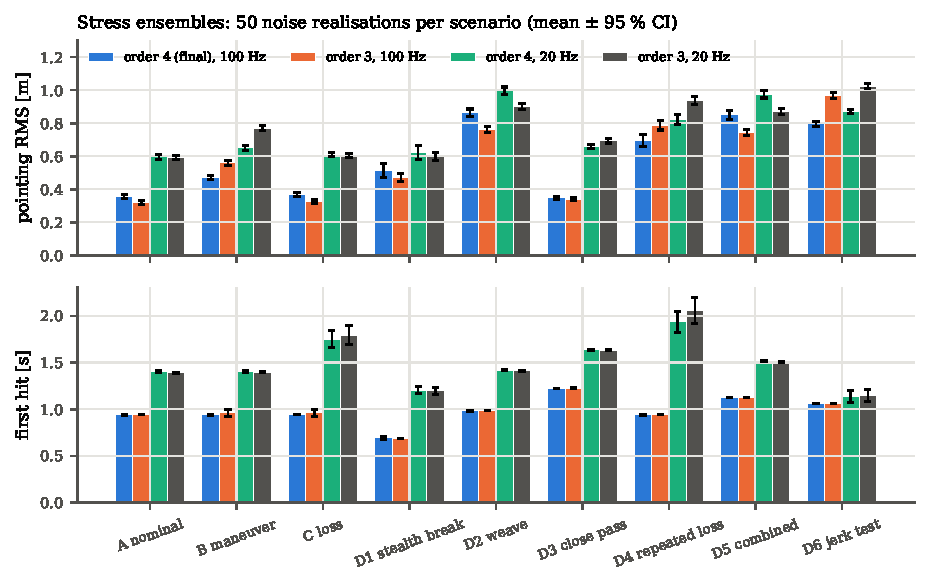
\includegraphics[width=\textwidth]{stress_per_scenario.pdf}
\caption{Per-scenario pointing RMS and first-hit time over 50 noise realisations (mean $\pm$ 95\% CI): order 4 (final) against order 3, at 100\,Hz and 20\,Hz.}
\label{fig:stress}
\end{figure}

\begin{table}[H]
\centering\small
\caption{Stress ensembles: 9 scenarios $\times$ 50 noise realisations.}
\label{tab:stress}
\begin{tabular}{lccccc}
\toprule
Variant & Intercepted & Pulse hit rate [95\% CI] & Misses & First hit [s] & Pointing RMS [m]\\
\midrule
Final (order 4), 100\,Hz & 450/450 & 99.90\% [99.75, 99.96] & 4 & 0.983 & 0.585\\
Order 3, 100\,Hz & 450/450 & 99.88\% [99.71, 99.95] & 5 & 0.988 & 0.586\\
Instant-fire 0.999 & 450/450 & 99.90\% [99.75, 99.96] & 4 & 1.013 & 0.585\\
Coast threshold 0.75 & 450/450 & 99.90\% [99.75, 99.96] & 4 & 0.983 & 0.585\\
Final (order 4), 20\,Hz & 450/450 & 99.61\% [99.35, 99.76] & 15 & 1.490 & 0.756\\
Order 3, 20\,Hz & 450/450 & 99.27\% [98.95, 99.50] & 28 & 1.504 & 0.777\\
\bottomrule
\end{tabular}
\end{table}

\obs{
\begin{itemize}
\item \textbf{Every engagement in every variant was intercepted.}
\item \textbf{Per-scenario pattern} (Fig.~\ref{fig:stress}): order 3 points better on smooth or weaving motion (A, C, D1, D2, D5; by 0.04--0.11\,m). Order 4 is better wherever the acceleration \emph{switches}: B by 0.09\,m, D4 by 0.09\,m, and the jerk test D6 by 0.17\,m. All of these differences have $p<0.005$.
\item \textbf{At 100\,Hz} the two orders tie on average ($\Delta$RMS $+0.002$\,m, $p=0.82$).
\item \textbf{At 20\,Hz}, where fewer corrections per radar sample amplify model mismatch, order 4 is significantly better overall: order 3 adds $+0.021$\,m RMS ($p=1.1\times10^{-4}$) and nearly doubles the misses (28 vs 15).
\item The stricter instant-fire threshold again only delays interception ($+0.029$\,s, $p=3\times10^{-33}$).
\item First hit is acquisition-limited in every scenario, except D4 at 20\,Hz, where the first blackout (1.0--1.5\,s) overlaps acquisition and pushes the first hit to about 1.9\,s.
\end{itemize}}
\takeaway{Order 4 is not uniformly better: on smooth targets order 3 is slightly more accurate. But order 4 wins exactly on the cases a hidden adversarial scenario is likely to contain (maneuver switches, high jerk, repeated loss) and at low controller rates. For an unseen evaluation, it is the robust choice (supports H3 in its robust form).}

% ==========================================================================================
\section{Results IV: Controller Rate, Timing and Implementation}
\begin{figure}[H]
\centering
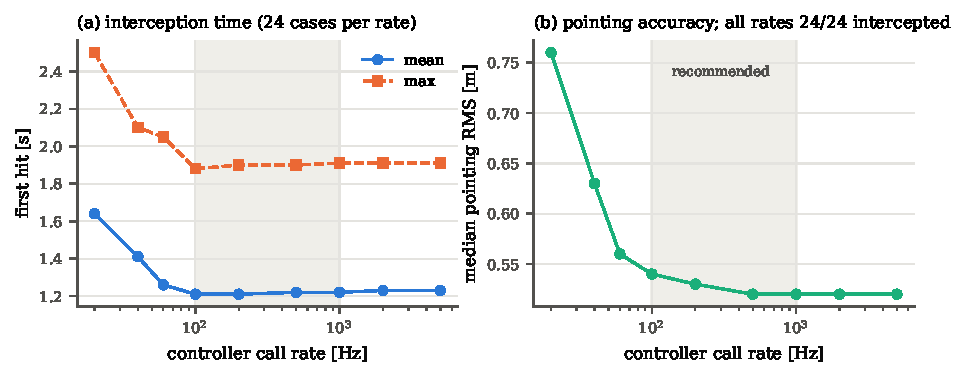
\includegraphics[width=\textwidth]{rate_study.pdf}
\caption{Interception time and pointing accuracy against controller call rate (24 cases per rate: A--D6 and 15 Monte Carlo seeds).}
\label{fig:rate}
\end{figure}

\begin{table}[H]
\centering\small
\caption{Controller-rate study.}
\label{tab:rate}
\begin{tabular}{rccccc}
\toprule
Rate [Hz] & Intercepted & Pulses hit & First hit mean / max [s] & Pointing RMS (median) [m]\\
\midrule
20 & 24/24 & 201/201 & 1.64 / 2.50 & 0.76\\
40 & 24/24 & 215/215 & 1.41 / 2.10 & 0.63\\
60 & 24/24 & 215/215 & 1.26 / 2.05 & 0.56\\
100 & 24/24 & 219/219 & 1.21 / 1.88 & 0.54\\
200 & 24/24 & 220/220 & 1.21 / 1.90 & 0.53\\
500 & 24/24 & 220/221 & 1.22 / 1.90 & 0.52\\
1000 & 24/24 & 220/221 & 1.22 / 1.91 & 0.52\\
2000 & 24/24 & 220/221 & 1.23 / 1.91 & 0.52\\
5000 & 24/24 & 220/221 & 1.23 / 1.91 & 0.52\\
\bottomrule
\end{tabular}
\end{table}

\obs{
\begin{itemize}
\item Every target is intercepted at every rate from 20\,Hz to 5\,kHz.
\item Performance improves up to about 100--200\,Hz and is flat above. The single miss at $\ge500$\,Hz is the D6 reversal shot of Section~5.
\item With forward-Euler plant integration at 1\,ms (controller 100\,Hz), Scenario B still intercepts at 0.95\,s. Forward Euler is unstable above 3.34\,ms because of the 8.9\,Hz mode, so the README requires a plant step of at most 1\,ms.
\item The MATLAB \texttt{turret\_controller.m} costs 0.51\,ms per call (median 0.33\,ms), so real-time use is practical up to about 1\,kHz.
\item Replaying 12 logged Python runs through the MATLAB controller reproduces the voltage within $3\times10^{-9}$\,V with identical fire commands, so the submitted code behaves exactly as the experiments report.
\end{itemize}}

% ==========================================================================================
\section{Results V: Robustness to the Evaluation Interface}
\label{sec:interface}
\textbf{What we did.} The instructor evaluates with his own script and hidden cases, which we never see. Besides unseen trajectories, the script may also deliver measurements and integrate the plant differently from our harness. We therefore ran the frozen design under eight plausible conventions, 300 engagements each on identical seeds:
\begin{itemize}
\item \textbf{I1} (reference): NaN with \texttt{meas\_valid}=0 between radar ticks, 100\,Hz.
\item \textbf{I2}: the last measurement \emph{held}, with \texttt{meas\_valid}=0 between ticks and during blackouts.
\item \textbf{I3}: the last measurement \emph{repeated with \texttt{meas\_valid}=1} on every call, including during blackouts (stale duplicates).
\item \textbf{I4, I5}: irregular radar timing, where a sample is taken at the call time once 50\,ms have elapsed, with call rates of 30\,Hz and 333\,Hz (steps that do not divide 50\,ms).
\item \textbf{I6}: the turret starting at a random angle $U(-10^\circ,85^\circ)$.
\item \textbf{I7}: forward-Euler plant integration at 1\,ms.
\item \textbf{I8}: the reference convention at 1\,kHz.
\end{itemize}

\begin{figure}[H]
\centering
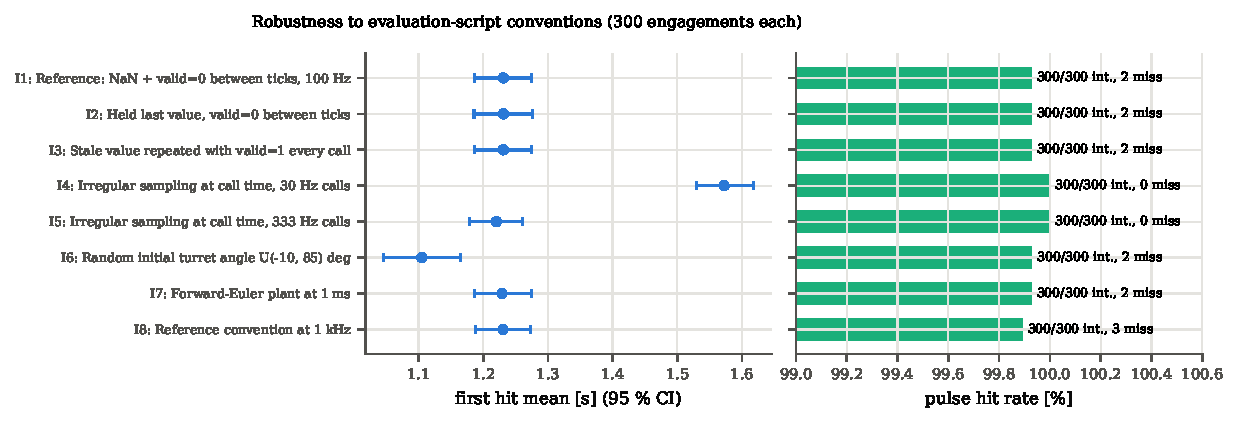
\includegraphics[width=\textwidth]{interface_robustness.pdf}
\caption{Frozen design under eight evaluation-script conventions (300 engagements each, identical seeds): mean first-hit time with 95\% CI, and pulse hit rate.}
\label{fig:interface}
\end{figure}

\begin{table}[H]
\centering\footnotesize
\caption{Robustness to evaluation-script conventions. $\Delta$ is paired against I1 (Wilcoxon $p$).}
\label{tab:interface}
\begin{tabularx}{\textwidth}{@{}lXcccc@{}}
\toprule
ID & Convention & Intercepted & Pulse hit rate (misses) & First hit mean / max [s] & $\Delta$ first hit [s], $p$\\
\midrule
I1 & reference, 100\,Hz & 300/300 & 99.93\% (2) & 1.231 / 2.05 & --\\
I2 & held value, \texttt{valid}=0 & 300/300 & 99.93\% (2) & 1.231 / 2.05 & 0, 1\\
I3 & stale value repeated, \texttt{valid}=1 & 300/300 & 99.93\% (2) & 1.231 / 2.05 & 0, 1\\
I4 & irregular sampling, 30\,Hz & 300/300 & 100.00\% (0) & 1.572 / 2.30 & $+0.341$, $7\times10^{-45}$\\
I5 & irregular sampling, 333\,Hz & 300/300 & 100.00\% (0) & 1.220 / 1.97 & $-0.011$, $10^{-25}$\\
I6 & random initial angle $-10^\circ$..$85^\circ$ & 300/300 & 99.93\% (2) & 1.105 / 2.80 & $-0.126$, $3\times10^{-4}$\\
I7 & forward-Euler plant, 1\,ms & 300/300 & 99.93\% (2) & 1.229 / 2.05 & $-0.002$, 0.99\\
I8 & reference, 1\,kHz & 300/300 & 99.89\% (3) & 1.231 / 1.96 & 0, --\\
\bottomrule
\end{tabularx}
\end{table}

\obs{
\begin{itemize}
\item \textbf{All 2\,400 engagements were intercepted} under every convention.
\item \textbf{Held or stale measurements are harmless.} I2 and I3 are bit-for-bit identical to I1, so the duplicate-measurement guard and the reliance on \texttt{meas\_valid} work. A script that keeps re-asserting \texttt{meas\_valid}=1 with an old sample, even through a blackout, cannot corrupt the track.
\item \textbf{Irregular radar timing is handled.} With samples taken whenever 50\,ms have elapsed, at call steps that do not divide 50\,ms (I4, I5), there were no misses at all. At 30\,Hz interception is 0.34\,s later, an effect of the coarse call rate (as in Section~8), not of the irregular timing. At 333\,Hz it matches the reference.
\item \textbf{Any initial turret angle works.} With the turret starting anywhere in $[-10^\circ,85^\circ]$ (I6), the worst first hit was 2.80\,s, consistent with the slew model of Section~\ref{sec:final}. The higher pointing RMS of this variant comes from 11 runs that started at $76^\circ$--$85^\circ$, whose long downward slews were still under way past the 2\,s mark where RMS starts counting.
\item \textbf{Plant integration and rate.} Forward-Euler at 1\,ms (I7) and a 1\,kHz call rate (I8) change nothing material.
\end{itemize}}
\takeaway{The design does not depend on our harness's conventions, so the unseen evaluation script should reproduce the performance reported here (supports H6).}


% ==========================================================================================
\section{Results VI: Prediction in the Loop and Homotopy-Guided Testing}
\label{sec:research}
% Results VI: prediction in the loop, the order-4 cap, shot-timed adversarial testing.
% Numbers: python/results/research/ (research_report.md, deconfound/, contact_order.md).
\textbf{Why this study.} A review of the frozen design raised two objections.
\begin{itemize}
\item \textbf{The prediction is cancelled trivially.} With deviation feedback the reference generator solves $(A_3+K)(\D)y_d=A_3(\D)\hat\theta+K(\D)\hat\theta$. On the estimator's polynomial nowcast this gives $(\D+20)^3(y_d-\hat\theta)=0$, whatever $A_3$ is. The Taylor polynomial agrees with $e^{st_p}$ only at $s=0$ in this loop (contact order 0), so the order-4 limit of Section~3.3 never binds.
\item \textbf{The homotopy idea was not implemented.} The hit probability used 17 hand-picked offsets, and the Monte Carlo drew random maneuvers instead of searching the directions that defeat the controller.
\end{itemize}
We therefore built every alternative behind a configuration flag, with the frozen design's defaults left untouched (bit-identical on all 1\,000 Monte Carlo seeds), and tested them on 1\,000 random and 1\,000 adversarial engagements each.

\subsection{Contact order: the order-4 cap, stated correctly}
\textbf{What we did.} We let the reference characteristic polynomial be $Q(x)=\sum_k q_kx^k$, $x=t_ps$, with $q_k=1/k!$ for $k\le m$, so $Q-e^x=O(x^{m+1})$ (\emph{contact order} $m$). We then added $f\le6$ free higher coefficients and maximised the least root damping $\zeta_{\min}$ by differential evolution.

\begin{figure}[H]
\centering
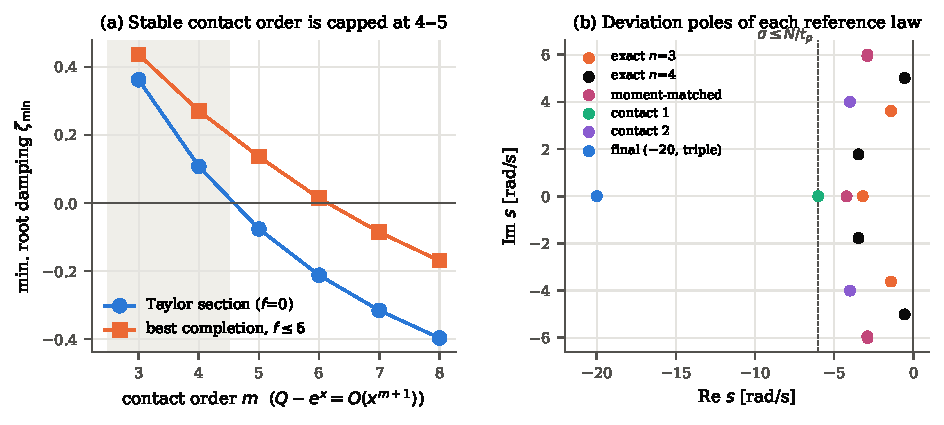
\includegraphics[width=\textwidth]{research_contact_order.pdf}
\caption{(a) Best least-root damping for each contact order. Pure Taylor sections (blue) are stable only up to order 4; extra free terms (orange) reach order 5 ($\zeta=0.136$) and order 6 only marginally ($\zeta=0.014$); no stable completion was found for orders 7--8. (b) Deviation poles of the reference laws tested. The dashed line is the decay bound $\sigma\le N/t_p=6$\,rad/s for a cubic that keeps the velocity prediction exact.}
\label{fig:contact}
\end{figure}

\obs{
\begin{itemize}
\item \textbf{The cap is real.} A stable loop can reproduce the $t_p$ shift to at most order 4--5 in $s$. Exact Taylor stops at $n=4$ with $\zeta=0.107$.
\item \textbf{Prediction in the loop is a choice of deviation poles.} In every mode the deviation obeys $P(\D)(y_d-\hat\theta)=0$, driven only by the estimator's correction at each radar update. Keeping first-order fidelity ($p_0=1$, $p_1=t_p$) forces $\sum 1/s_i=-t_p$, so the slowest pole decays at no more than $N/t_p$ (6\,rad/s for a cubic). The frozen design gives up that fidelity to place its poles at $-20$\,rad/s.
\item We tested six such laws: exact Taylor $n=3$ and $n=4$ ($T=1/A_n$); a moment-matched quintic $Q=A_3+0.741x^4/24+0.470x^5/120$, which keeps order-3 contact and whose two free coefficients maximise the slowest decay (2.9\,rad/s); contact order 1, $(1+s/6)^3$, which keeps only the velocity term and attains the bound; contact order 2, $((s^2+8s+32)/32)^2$; and blends of $A_3$ with the frozen design.
\item \textbf{Same large-signal handling for all.} Every law uses the frozen design's saturated acquisition cascade outside a hysteretic band and switches to its own linear law inside it ($|y_d-\hat\theta|<3$\,mrad and $|\dot y_d-\hat\theta'|<0.02$\,rad/s to enter, $>15$\,mrad to leave). No law is penalised by an unsaturated slew transient or by its initialisation.
\end{itemize}}
\takeaway{The order-4 limit binds on the \emph{transient} of the tracking loop, not on its steady state. It restricts which deviation poles may be chosen if the loop is to keep the Taylor prediction; it does not change what the turret tracks in steady state.}

\subsection{Shot-timed adversarial testing}
\textbf{What we did.} We work in the plane $(t,e)$, where $e$ is the target's signed cross-range offset from the beam. The obstacles are the firing events, the tubes $\{t_k\}\times[-\Reng,\Reng]$. A target path is a graph $e(t)$, so in this one-dimensional setting its class reduces to the sign of $e$ at each event, $h_k\in\{+1,0,-1\}$ (above, through = hit, below): the 1-D analogue of the homotopy classes of T-MPC \cite{degroot2024tmpc}, not a topological search in a richer space. The adversary \texttt{HG<seed>} takes a random base engagement and finds the frozen design's firing times. Before each event it reverses the normal acceleration at the envelope limit, with quintic ramps, toward the side that class \texttt{seed}\,\%\,5 requires (above, below, cross-down, cross-up, alternating). It chooses the lead time that maximises the frozen design's mean miss, and re-simulates once to check that the shots have not moved (a fixed-point step). The adversary is therefore white-box and non-causal: it knows the controller's shot times, which a real target cannot. All 1\,000 cases respect the envelope and the blackout rules.

\obs{
\begin{itemize}
\item \textbf{The classes steer the misses.} Where the frozen design misses, the side follows the attack: ``above'' seeds miss 38 above and 4 below, ``below'' seeds 1 above and 31 below.
\item \textbf{The adversary is weak.} Even with the shot times known, 633 of 1\,000 cases still had every pulse ``through'', and only 116 realised the intended class. All 1\,000 were intercepted.
\item The adversarial family is therefore worst-case evidence about \emph{where} misses come from. It is never pooled into the failure bound.
\end{itemize}}

\subsection{Results: nominal accuracy against adversarial robustness}
\begin{table}[H]
\centering\small
\caption{Reference laws on 1\,000 random (MC) and 1\,000 adversarial (HG) engagements, controller at 100\,Hz. Every configuration intercepted 1\,000/1\,000 in both families. ``Hits'' = pulses that hit. Exact $n=4$ uses an order-5 estimator ($\sigma=150$, $\tau=0.2$, not optimised).}
\label{tab:research}
\begin{tabular}{@{}lrrrrrr@{}}
\toprule
& \multicolumn{3}{c}{MC0--999} & \multicolumn{3}{c}{HG0--999}\\
\cmidrule(lr){2-4}\cmidrule(l){5-7}
Design & RMS [m] & misses & hits & RMS [m] & miss rate & hits\\
\midrule
\textbf{Frozen design} & \textbf{0.56} & \textbf{4} & \textbf{9193} & \textbf{1.21} & 2.67\% & \textbf{8901}\\
Blend $\alpha=0.2$ & 0.65 & 7 & 9187 & 1.41 & 3.57\% & 8697\\
Contact order 1 & 0.99 & 24 & 8907 & 1.90 & 1.08\% & 8515\\
Contact order 2 & 1.82 & 18 & 8443 & 3.09 & 1.08\% & 8116\\
Exact Taylor $n=3$ & 2.82 & 23 & 8033 & 3.83 & 0.94\% & 7802\\
Moment-matched & 2.94 & 33 & 7904 & 4.78 & 1.09\% & 7776\\
Exact Taylor $n=4$ & 4.91 & 23 & 7440 & 6.26 & 0.39\% & 7459\\
\bottomrule
\end{tabular}
\end{table}

\begin{figure}[H]
\centering
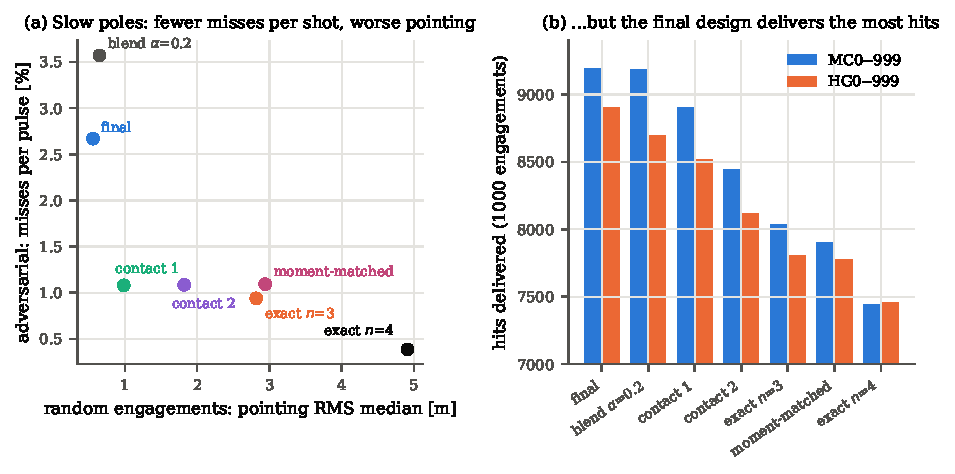
\includegraphics[width=\textwidth]{research_tradeoff.pdf}
\caption{(a) Nominal pointing error against the adversarial miss rate per pulse. (b) Hits delivered in each family. Slow deviation poles miss less often per shot, but they shoot less and hit less.}
\label{fig:tradeoff}
\end{figure}

\obs{
\begin{itemize}
\item \textbf{On random engagements the frozen design is best on every measure.} Every slower design has worse pointing (paired $p<10^{-160}$, Holm). The exact, moment-matched and contact-order laws also miss more (18--33 against 4, $p\le0.04$, Holm). The blends with $\alpha\ge0.1$ are not significantly different in misses.
\item \textbf{Under attack the per-pulse miss rate ranks the other way.} Slow poles miss 60--85\% fewer pulses per shot, because the 20\,rad/s loop chases each estimator correction and turns the lag the adversary induces into beam motion at the shot.
\item \textbf{But the frozen design still delivers the most hits.} The slow designs are on target 26--65\% of the time instead of 93\%, so the hit-probability gate holds their shots back. Time to first hit, which decides an interception, is within about 50\,ms for all designs.
\end{itemize}}

\subsection{Without the acquisition slew}
\textbf{What we did.} To check that the slow laws are not judged only on acquisition, we started the turret on the target's initial elevation (no slew) and re-ran seeds MC0--299 for the frozen design, exact Taylor $n=3$, contact order 1 and moment-matched.

\begin{table}[H]
\centering\small
\caption{No-slew start against the standard $0^\circ$ start, MC0--299 (pointing RMS median; misses / pulses).}
\label{tab:noslew}
\begin{tabular}{@{}lrrrr@{}}
\toprule
& \multicolumn{2}{c}{$0^\circ$ start} & \multicolumn{2}{c}{no slew}\\
\cmidrule(lr){2-3}\cmidrule(l){4-5}
Design & RMS [m] & misses & RMS [m] & misses\\
\midrule
\textbf{Frozen design} & \textbf{0.56} & 2 / 2752 & \textbf{0.52} & 1 / 3000\\
Contact order 1 & 0.98 & 5 / 2674 & 0.84 & 5 / 2781\\
Exact Taylor $n=3$ & 2.84 & 6 / 2415 & 1.31 & 7 / 2648\\
Moment-matched & 2.96 & 11 / 2384 & 1.69 & 7 / 2607\\
\bottomrule
\end{tabular}
\end{table}

\obs{
\begin{itemize}
\item Removing the slew halves the error of the exact and moment-matched laws, so part of their penalty is acquisition.
\item They still point 1.6--3.2 times worse than the frozen design, which barely changes. The remaining penalty is the slow deviation poles following the estimator's corrections, not initialisation or ringing from the slew.
\end{itemize}}

\subsection{Does the robustness survive an adversary tuned against each design?}
We re-ran the adversarial search against contact order 1 and exact Taylor $n=3$ on seeds 0--199, and played every adversary against every design (Fig.~\ref{fig:deconf}).

\begin{figure}[H]
\centering
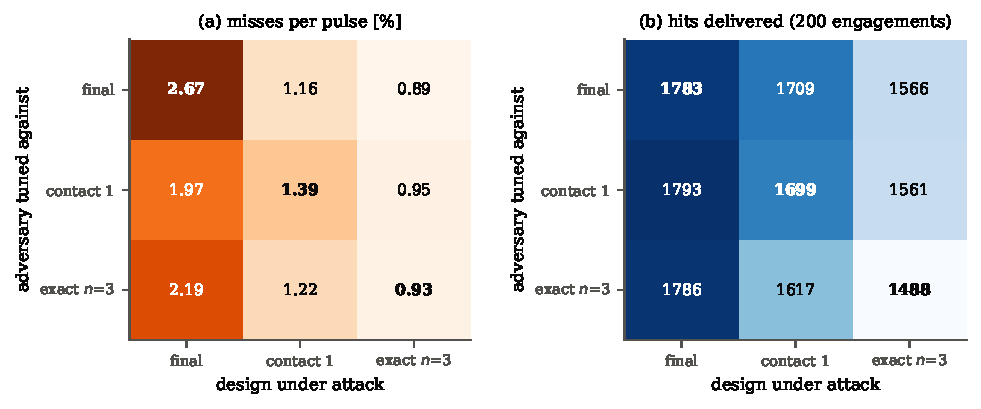
\includegraphics[width=\textwidth]{research_deconfound.pdf}
\caption{Attacker $\times$ defender on 200 engagements. Bold: each design against the adversary tuned on it. All 1\,800 engagements were intercepted.}
\label{fig:deconf}
\end{figure}

\obs{
\begin{itemize}
\item Each design is hit hardest by its own adversary (the diagonal). Its worst-case miss rate is 2.67\% for the frozen design, 1.39\% for contact order 1 and 0.93\% for exact Taylor $n=3$.
\item Exact Taylor $n=3$ beats the frozen design's miss rate under every adversary ($p\le0.008$). Contact order 1's advantage is not significant under its own adversary (36 vs 24 misses, $p=0.15$).
\item In hits delivered the frozen design wins every cell.
\end{itemize}}

\subsection{Homotopy fire planner and the remaining audit items}
\begin{itemize}
\item \textbf{Fire planner.} The planner uses 25 maneuver hypotheses scored by their sign pattern over the remaining recharge window, Gaussian spread from the noise-free covariance, and the plan-consistency rule of T-MPC \cite{degroot2024tmpc}. It hits 19\,ms earlier on random engagements but misses more there ($4\to11$) and fewer under attack ($244\to230$), neither significantly. It was not adopted; the mixture rule stays.
\item \textbf{Hit-probability calibration under attack.} On random engagements $\Phit$ at the pulses is calibrated (mean 99.91\% predicted, 99.96\% observed over 9\,197 pulses). Under the adversary it is overconfident: 99.74\% predicted against 97.33\% observed over 9\,145 pulses, and in the 0.95--0.99 bin 97.0\% against 64.1\% (117 pulses). The 17 maneuver classes hedge a constant acceleration since the last radar sample, not a reversal timed to the shot.
\item \textbf{Plant error.} With $R$, $L$, $J_{eq}$ and $b$ each drawn in $\pm20\%$ per engagement (controller nominal), the frozen design intercepted 1\,000/1\,000 with 6 misses in 9\,190 pulses and unchanged pointing (0.557\,m). These four parameters barely enter the feed-forward, whose dominant term $1001.5\,\dot y_d=(Rb+N^2K_tK_e)/(NK_t)\,\dot y_d\approx NK_e\,\dot y_d$ is set by the back-EMF constant. We therefore re-ran with all six parameters, $K_t$ and $K_e$ included (Table~\ref{tab:pert6}).

\begin{table}[H]
\centering\small
\caption{Six-parameter plant error ($R,L,J_{eq},b,K_t,K_e$ each $U(0.8,1.2)$), MC0--999, binned by the $K_e$ factor.}
\label{tab:pert6}
\begin{tabular}{@{}lrrr@{}}
\toprule
$K_e$ factor & runs & RMS median [m] & misses\\
\midrule
0.80--0.90 & 240 & 3.16 & 7\\
0.90--0.95 & 142 & 1.94 & 1\\
0.95--1.05 & 261 & 0.77 & 3\\
1.05--1.10 & 114 & 1.55 & 2\\
1.10--1.20 & 243 & 3.27 & 2\\
\midrule
all & 1\,000 & 1.69 & 15 / 8\,158\\
\bottomrule
\end{tabular}
\end{table}
All 1\,000 were intercepted and 99.82\% of pulses hit, but pointing RMS rose from 0.56 to 1.69\,m (paired $p<10^{-160}$), fewer pulses were fired (8\,158 against 9\,190) and the mean first hit was 0.18\,s later. The error correlates with $|\log K_e|$ (Spearman $\rho=0.71$) and hardly with $K_t$ ($\rho=0.04$), as the feed-forward predicts. The design is robust in interception but its accuracy depends on knowing $K_e$. Friction and backlash are not modelled and were not tested.
\item \textbf{Re-identification.} Removing it changed nothing measurable (MC 3 vs 4 misses, HG 245 vs 244).
\item \textbf{Envelope projection} activates in 44\% of random and 96\% of adversarial engagements (0.9 and 12 times per run), always on the acceleration estimate.
\end{itemize}

\takeaway{The order-4 cap and the shot-timed adversary are now real parts of the analysis, and both were tested. Neither overturns the frozen design, but the adversary exposes an overconfident $\Phit$ and the plant study a sensitivity to $K_e$. Keeping the Taylor prediction in the loop forces slow deviation poles, which cost far more pointing accuracy and hits than they save in per-shot misses under attack. The frozen design remains the submitted one.}


% ==========================================================================================
\section{Final Evaluation: Expected Performance on Unseen Cases}
\label{sec:final}
The instructor's evaluation cases are hidden, and the design was frozen before any of them could be seen. This section therefore states, from our own evidence, what the frozen design should be expected to do on them, and where the expectation stops.

\subsection{What the hidden cases share with our tests}
The specification guarantees that every evaluation case satisfies:
\begin{itemize}
\item the operating envelope: $800\le r\le2000$\,m, $|\mathbf v|\le150$\,m/s, $|\mathbf a|\le20$\,m/s$^2$, with smooth bounded maneuvers in $x$ and $y$;
\item measurement-loss bounds: onset at or after 1\,s and duration at most 0.5\,s.
\end{itemize}
Our tests cover that envelope from four directions:
\begin{itemize}
\item random sampling across it (1\,000 + 500 + 500 engagements, Fig.~\ref{fig:mcfeat});
\item deliberately adversarial corners (D1--D6, each with 50 noise realisations): maneuvering inside a blackout, near-$a_{\max}$ weaving, a close pass to $83^\circ$, four blackouts, and 450\,m/s$^3$ jerk;
\item 1\,000 homotopy-guided adversarial engagements that reverse the target's maneuver just before each shot (Section~\ref{sec:research});
\item eight evaluation-script conventions (Section~\ref{sec:interface}).
\end{itemize}
No parameter was tuned per scenario. One parameter set was used for all of them.

\subsection{Quantitative expectations}
\begin{enumerate}
\item \textbf{Interception.} The failure bound rests on the \textbf{1\,000 independent random engagements} only: all were intercepted, so the probability of failing to intercept an admissible engagement is below \textbf{0.38\%} (one-sided 97.5\% Wilson; the rule of three gives 0.30\%). The other runs are not pooled into this bound, because they reuse the same trajectories (20\,Hz, $60^\circ$ start, interface conventions, plant error) or are noise replicas of nine scenarios (stress ensembles). They intercepted every case too, as did the 1\,000 adversarial engagements, which are worst-case evidence and not a random sample.
\item \textbf{Interception time.} This is predictable from geometry (Fig.~\ref{fig:fh}b):
\[ t_{\mathrm{hit}} \approx 0.26 + 0.0296\times\big|\theta_T(0)-\theta_{\mathrm{turret}}(0)\big|_{\mathrm{deg}}\ \mathrm{s}\ \ (\pm0.20\,\mathrm s,\ 95\%). \]
For a turret starting at $0^\circ$ and targets between $8^\circ$ and $55^\circ$, expect 0.5--1.9\,s (mean about 1.2\,s). The worst conceivable slew, $95^\circ$ from $-10^\circ$ to $+85^\circ$, gives about 3.1\,s. A blackout overlapping acquisition delays the first hit until after recovery, by up to 0.5\,s.
\item \textbf{Engagement accuracy.} Expect a pulse hit rate of 99.8--99.99\% at 100\,Hz--1\,kHz, and about 99.6--99.8\% at 20\,Hz. Typical pulses land 0.4\,m from the target (99th percentile 1.5\,m).
\item \textbf{Consistency across cases.} Pointing RMS varies smoothly with maneuver intensity (0.3--0.6\,m on gentle targets, 0.8--1.0\,m on near-$a_{\max}$ weaves). Its 95th percentile over all Monte Carlo engagements is 0.83\,m. No case type produced a qualitatively different failure mode.
\end{enumerate}

\subsection{Interface requirements the evaluation script must meet}
\begin{itemize}
\item Plant integration with a step $\le1$\,ms, or \texttt{ode45}. With larger forward-Euler steps the \emph{plant itself} becomes numerically unstable.
\item Controller called at $\ge20$\,Hz; 100\,Hz--1\,kHz is recommended. Any step works, because the controller reads $\Delta t$ from $t$.
\item Nothing else is needed. The controller resets itself when $t$ decreases or $t=0$, ignores non-new or NaN measurements, and works from any initial turret angle.
\end{itemize}

\subsection{Where the evidence stops}
The expectations above hold for admissible engagements as specified. They are not evidence for:
\begin{itemize}
\item maneuvers sharper than tested (jerk above about 450\,m/s$^3$, i.e.\ near-instant acceleration switches);
\item blackouts longer than 0.5\,s, after which drift exceeds $\Reng$ for any controller;
\item targets above the $+85^\circ$ elevation stop, which are mechanically unreachable;
\item a plant that differs from the specified one by more than $\pm20\%$ in $R$, $L$, $J_{eq}$ or $b$ (tested: 1\,000/1\,000 intercepted, unchanged accuracy). Beyond that, robustness rests on the analytical margins (PM $68^\circ$, GM 16\,dB, $M_s=1.21$).
\end{itemize}

% ==========================================================================================
\section{Verdicts and Conclusions}
\label{sec:verdict}

\begin{table}[H]
\centering\small
\caption{Verdict on each hypothesis of Section~\ref{sec:thesis}.}
\label{tab:verdict}
\begin{tabularx}{\textwidth}{@{}lXl@{}}
\toprule
& Evidence & Verdict\\
\midrule
H1 & Turret sits on the true elevation while the reference leads by $t_p$ (Section~5). Pointing error (0.2--0.4\,m) matches estimation error (0.22\,m median). $\theta-y_d$ is under 3\,cm. The return to the nowcast holds for any stable deviation poles; keeping the Taylor prediction in the loop is possible only to order 4--5 and costs accuracy (Section~\ref{sec:research}). & \textbf{Supported}\\
H2 & $E[z^2]=1.008$ tracking, 0.92 coasting. Calibrated $\Phit$ (Brier 0.0045). 4 misses observed vs 8.6 predicted. & \textbf{Supported}\\
H3 & Order 2: 3 interceptions lost and 34$\times$ the misses. Order 4 vs 3: better on maneuver switches (B, D4, D6) and at 20\,Hz; slightly worse on smooth targets. & \textbf{Partly supported:} necessary vs order 2; vs order 3 a trade-off, not uniformly better\\
H4 & 99.96\% pulse accuracy. Cadence at the recharge limit (median gap 1.01\,s). D2 shows fire withheld at bad moments. 0.999 threshold only slower. & \textbf{Supported}\\
H5 & Graceful degradation (median 0.8\,m peak), honest $\sigma$ growth, 0.4\,s recovery. No late blind shots. Coasting shots 211/211 hit. & \textbf{Supported}\\
H6 & 1\,000/1\,000 independent random interceptions (failure $<0.38\%$); 1\,000/1\,000 adversarial; $\pm20\%$ plant error harmless; geometry-predictable timing; robust to eight interface conventions. & \textbf{Supported within the envelope}\\
\bottomrule
\end{tabularx}
\end{table}

\paragraph{Conclusion.} The evidence supports the thesis.
\begin{itemize}
\item Treating the prescribed prediction horizon as a lag to be cancelled, rather than a lead to be applied, yields a design in which the turret tracks the target's \emph{present} elevation. Keeping the Taylor prediction itself inside the loop is bounded at order four by the stability of the Taylor sections and forces slow deviation poles. We tested that route, and it costs more accuracy and more hits than it saves.
\item Pointing error is then limited only by estimation, about 0.2--0.4\,m against a 2\,m engagement radius.
\item A jerk-state estimator matched to the plant's relative degree, an exact plant-inverse feed-forward and a calibrated firing rule turn that accuracy into hits: 99.96\% of pulses, with interception time set by turret kinematics alone.
\item The same frozen design intercepted all 1\,000 independent random engagements (failure below 0.38\%) and all 1\,000 homotopy-guided adversarial ones. It is insensitive to $\pm20\%$ plant error and to how an evaluation script delivers measurements.
\item Under the adversary its per-pulse miss rate rises to 2.7\%, because its fast deviation poles follow each estimator correction. Designs with slower poles miss less per shot but shoot and hit less, so the frozen design still delivers the most hits.
\end{itemize}
Four of our own ideas, the ambush hold, class re-identification, the Taylor-prediction-in-the-loop reference laws and the homotopy fire planner, were tested and discarded or demoted by the same evidence. The order-4 choice is justified by robustness on maneuver switches, not by uniform superiority. The design's limits are those of physics, not of the controller: turret slew rate bounds interception time, and the reachable set of a maneuvering target bounds what any controller can guarantee late in a long blackout.

\appendix
\section{Reproducing This Report}
\begin{verbatim}
cd python
bash scripts/run_all_experiments.sh       # all core experiments
python scripts/interface_robustness.py --n 300
python scripts/plot_report_extras.py
python scripts/research_contact_order.py  # Section 10: contact order
sh scripts/run_research.sh                # HG cache + MC/HG campaign
sh scripts/run_research2.sh && sh scripts/run_deconfound.sh
python scripts/research_eval.py && python scripts/research_deconfound.py
python scripts/plot_research.py
# MATLAB (matlab/): parity_check, time_controller, run_scenarios
\end{verbatim}
Raw results are written to \texttt{python/results/}: the Monte Carlo statistics, the stress and interface reports, and the rate-study table.

\end{document}
